\chapter{从强子Regge轨迹到光锥弦}

\lectureoverview{弦理论最初并不是作为量子引力理论而诞生的。它起初是为了理解强子的谱与散射。笔直的Regge轨迹暗示存在一个延展客体；{\proseunicodefont π}介子--{\proseunicodefont π}介子散射中的对偶性则暗示，两个表面上不同的过程其实是同一曲面的两种切片方式。我们将沿着这些线索进入世界面图像，把强子弦重新解释为QCD流管，然后利用无限动量参照系推导开弦的横向力学。核心结果是，其有效内部哈密顿量度量的是质量的平方。因此，在该描述中与\(L^2\)成正比的胡克定律能量，就变成与\(L\)成正比的静止能量，这正是具有恒定张力的弦的定义性行为。}

\section{弦理论的强子起源}

大约在1968--1970年，导致弦理论出现的问题涉及质子、中子，尤其是介子。夸克模型当时已经是一个严肃的想法，但强子的夸克组分尚未以现代意义在实验上得到确立。胶子在通常讨论中的地位就更不显著了。南部曾提出过相关的规范场思想，但量子色动力学的成熟语言当时还不存在。当时的原材料反而是强相互作用粒子异常丰富的谱。

暂时忽略质子--中子的区分，把两种状态都称为核子，这是有用的。核子之外还有自旋更大的更重状态，接着是自旋更大的更重状态。Chew和Frautschi把这样的族组织在一张图上，纵轴是角动量，横轴是质量的平方。按当时的历史单位，质子质量约为1 BeV；同一单位现在称为GeV。

以\(\hbar\)为单位来度量角动量。对于重子族，无量纲自旋值为半整数，

\begin{equation}
  J=\frac12,\frac32,\frac52,\ldots,
\end{equation}

而介子族具有整数自旋。引人注目的经验事实是，无论哪一族，当以\(M^2\)为横轴作图时，都近似落在一条直线上。用现代记号可写为

\begin{equation}
  J\simeq \alpha_0+\alpha' M^2,
  \label{eq:l01-regge-trajectory}
\end{equation}

其中\(\alpha_0\)是截距，\(\alpha'\)是Regge斜率。\editorialnote{本讲强调所观测到的线性关系及其近乎普适的斜率。引入截距记号只是为了紧凑地陈述该关系；这些轨迹是经验的、近似的。}

最初的直线并不令人信服，因为它只经过两个已知点。任意两点都确定一条直线。令人惊讶的是后来发生的事：新发现的状态继续落在同一条直线附近。介子轨迹也显示出同样的组织方式。{\proseunicodefont π}介子从\(J=0\)附近开始，在GeV尺度上质量很小；{\proseunicodefont ρ}介子从\(J=1\)开始；进一步的激发继续向上延伸。一个族中可能出现五、六或七个状态。更引人注目的是，不同的重子和介子轨迹几乎平行。因此，角动量增加一个量子，对应着质量的平方增加大致相同的量：

\begin{equation}
  \Delta J=1
  \quad\Longrightarrow\quad
  \Delta M^2\simeq \frac{1}{\alpha'}.
  \label{eq:l01-regge-spacing}
\end{equation}

\begin{classroomqa}
\audiencequestion{不同的Regge轨迹平行意味着什么？\lecturetimestamp{00:09:32}}
\lecturerresponse{选取一族粒子，画出它的所有激发态；它们落在一条直线上。对另一个介子族或重子族重复这一做法。即使截距不同，这些直线也具有大致相同的斜率。因此，角动量增加相同的量，所付出的\(M^2\)增量也大致相同。这一共同的斜率被称为普适Regge斜率。}
\end{classroomqa}

与普通延展客体的比较说明了这一模式为何重要。篮球被旋转时会获得转动能量，但它的轨迹是弯曲的而非直线的，而且在角速度足够高时，球会被撕裂。原子也有转动激发，但最终会被电离；它的轨迹会终止。强子则显示出简单得多的序列，而且在现有数据范围内，没有迹象表明该序列会终止。

这一谱表明，强子的行为不像一个点。点没有可供旋转或形变的空间结构。电子没有观测到更高自旋内部态的塔，因而在目前的实验界限内是类点的。相比之下，强子可以被旋转起来。它的谱暗示了复合性，而自旋与质量之间的关系则暗示，该客体随着角动量增加而发生形变。

\section{{\proseunicodefont π}介子--{\proseunicodefont π}介子散射中的对偶性}

光谱学提供了一条线索。{\proseunicodefont π}--{\proseunicodefont π}散射提供了另一条线索。两个{\proseunicodefont π}介子可以结合成一个类{\proseunicodefont ρ}共振态，随后又作为两个{\proseunicodefont π}介子重新出现。在传统的费曼图中，这是一个湮灭与再产生过程，习惯上称为\(s\)道过程。把同一个基本图旋转过来，就得到一个交叉的，即\(t\)道过程，其中{\proseunicodefont π}介子之间交换了一个类{\proseunicodefont ρ}粒子。

{\proseunicodefont ρ}并不孤单。它属于一个Regge族，因此自洽性似乎要求在两个道中都包含{\proseunicodefont ρ}及其所有激发伙伴。示意地，

\begin{equation}
  \mathcal A(s,t)\simeq
  \sum_n \mathcal A^{(s)}_{\rho_n}(s,t),
  \qquad
  \mathcal A(s,t)\simeq
  \sum_n \mathcal A^{(t)}_{\rho_n}(s,t).
  \label{eq:l01-channel-sums}
\end{equation}

这些表达式并不是两个应当简单相加的近似。数值研究发现，在湮灭道中对共振塔求和，已经给出了大致相当于交换道所预期的贡献。反过来，交换的塔也能重现共振描述。因此，把两个完整的塔相加，似乎把同一物理计算了两次。通常的微扰记账法说，如果两个图存在，就必须都包括进来。而强子振幅却暗示，这两种道的描述是对偶的。

\begin{figure}[H]
  \centering
  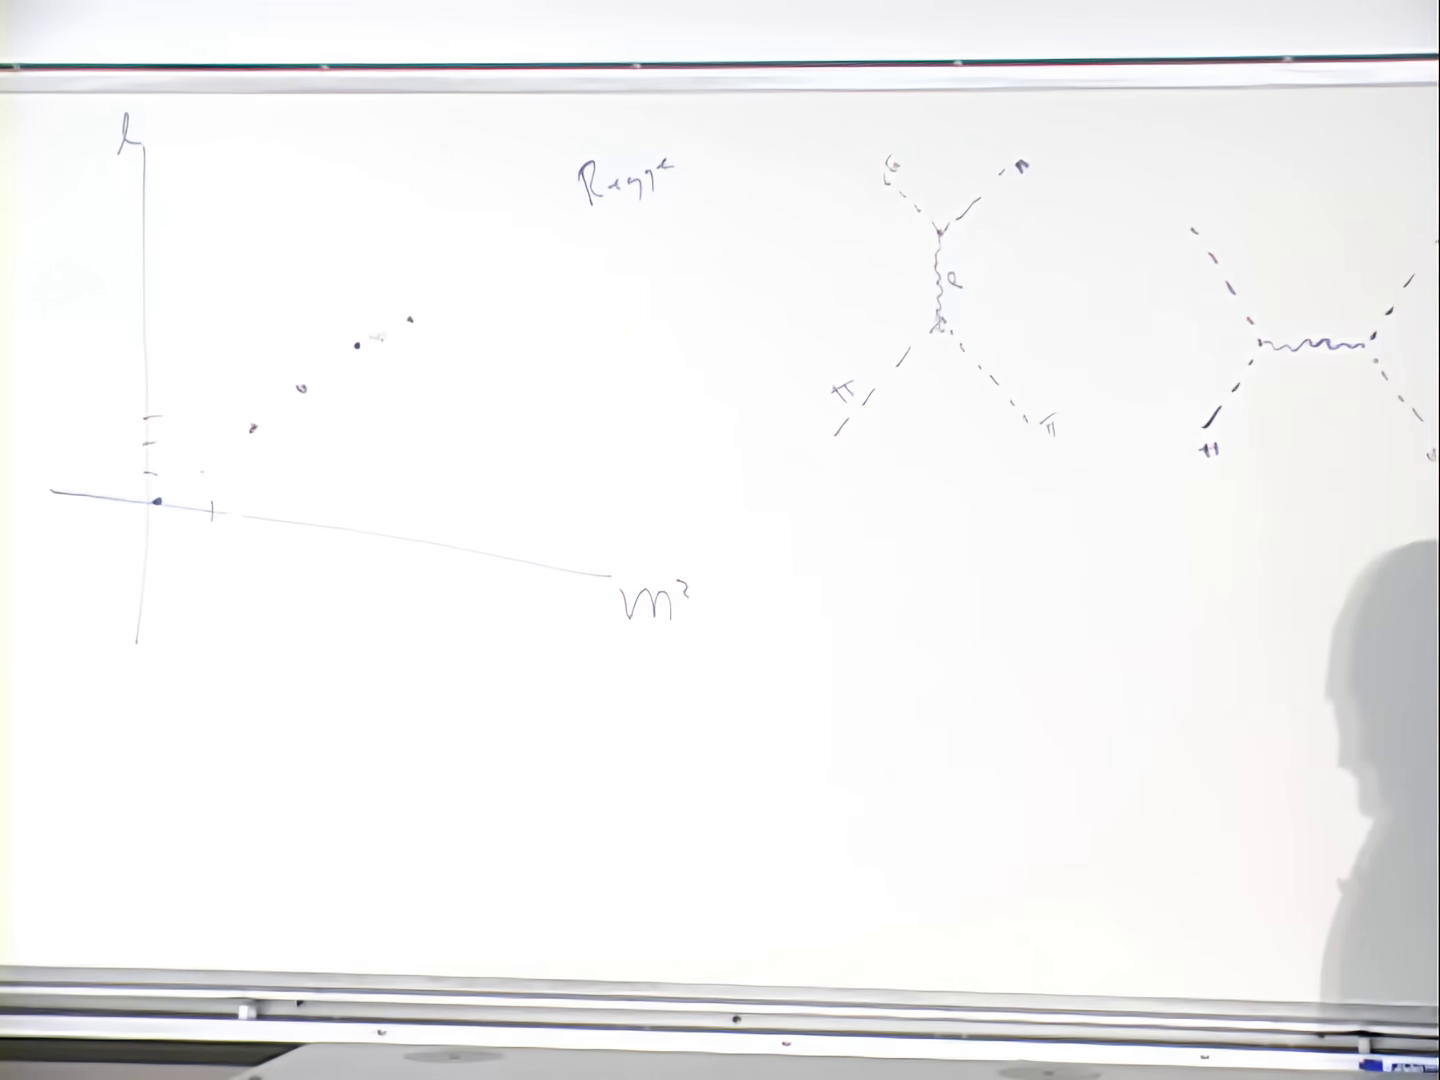
\includegraphics[width=0.82\textwidth]{lecture_01_figure_01.png}
  \caption{这张图把Chew--Frautschi图与湮灭道和交叉道图联系起来，使光谱线索和散射线索成为同一个问题的一部分。}
  \lectureframe{00:14:20}
  \label{fig:l01-regge-duality-board}
\end{figure}

同样的关系可以分离成一个清晰的示意图。第一个面板记录了线性谱；另外两个表示同一振幅的另一种道展开。

\begin{figure}[H]
  \centering
  \resizebox{\textwidth}{!}{%
  \begin{tikzpicture}[>=Latex,thick]
    \begin{scope}
      \draw[->] (0,0) -- (4.2,0) node[right] {$M^2$};
      \draw[->] (0,0) -- (0,3.4) node[above] {$J$};
      \draw[blue!65!black] (0.45,0.35) -- (3.55,2.95);
      \draw[orange!80!black] (0.75,0.20) -- (3.85,2.80);
      \foreach \x/\y in {0.65/0.52,1.35/1.10,2.05/1.69,2.75/2.27,3.45/2.86}
        \fill[blue!65!black] (\x,\y) circle (0.07);
      \foreach \x/\y in {0.95/0.37,1.65/0.95,2.35/1.54,3.05/2.12,3.75/2.71}
        \fill[orange!80!black] (\x,\y) circle (0.07);
      \node at (2.1,-0.55) {parallel Regge families};
    \end{scope}
    \begin{scope}[xshift=5.7cm]
      \draw[->] (-1.5,1.2) -- (-0.3,0.25);
      \draw[->] (-1.5,-1.2) -- (-0.3,-0.25);
      \draw[decorate,decoration={snake,amplitude=1.5pt,segment length=7pt}]
        (0,0.25) -- (0,-0.25);
      \draw[->] (0.3,0.25) -- (1.5,1.2);
      \draw[->] (0.3,-0.25) -- (1.5,-1.2);
      \node at (0,-1.75) {$s$-channel tower};
    \end{scope}
    \begin{scope}[xshift=10.5cm]
      \draw[->] (-1.5,1.2) -- (1.5,1.2);
      \draw[->] (-1.5,-1.2) -- (1.5,-1.2);
      \draw[decorate,decoration={snake,amplitude=1.5pt,segment length=7pt}]
        (0,0.95) -- (0,-0.95);
      \node at (0,-1.75) {$t$-channel tower};
    \end{scope}
  \end{tikzpicture}}
  \caption{平行的Regge族以及强子对偶中涉及的两种道展开。}
  \label{fig:l01-regge-duality-redraw}
\end{figure}

\section{一个世界面，两种切片方式}

自然的回应是寻找一段可以用两种方式解读的几何历史。用夸克--反夸克对表示一个{\proseunicodefont π}介子，并让时间向上流动。不要只画一维的粒子线，而是填充由夸克轨迹围成的区域。对这一二维历史作水平切片，可能显示两条入射弦结合，随后又分开。换一种切片方式，则显示一条弦从一侧交换到另一侧。这两幅费曼道图像不再是彼此独立的机制；它们是同一个曲面的不同分解。

\begin{figure}[H]
  \centering
  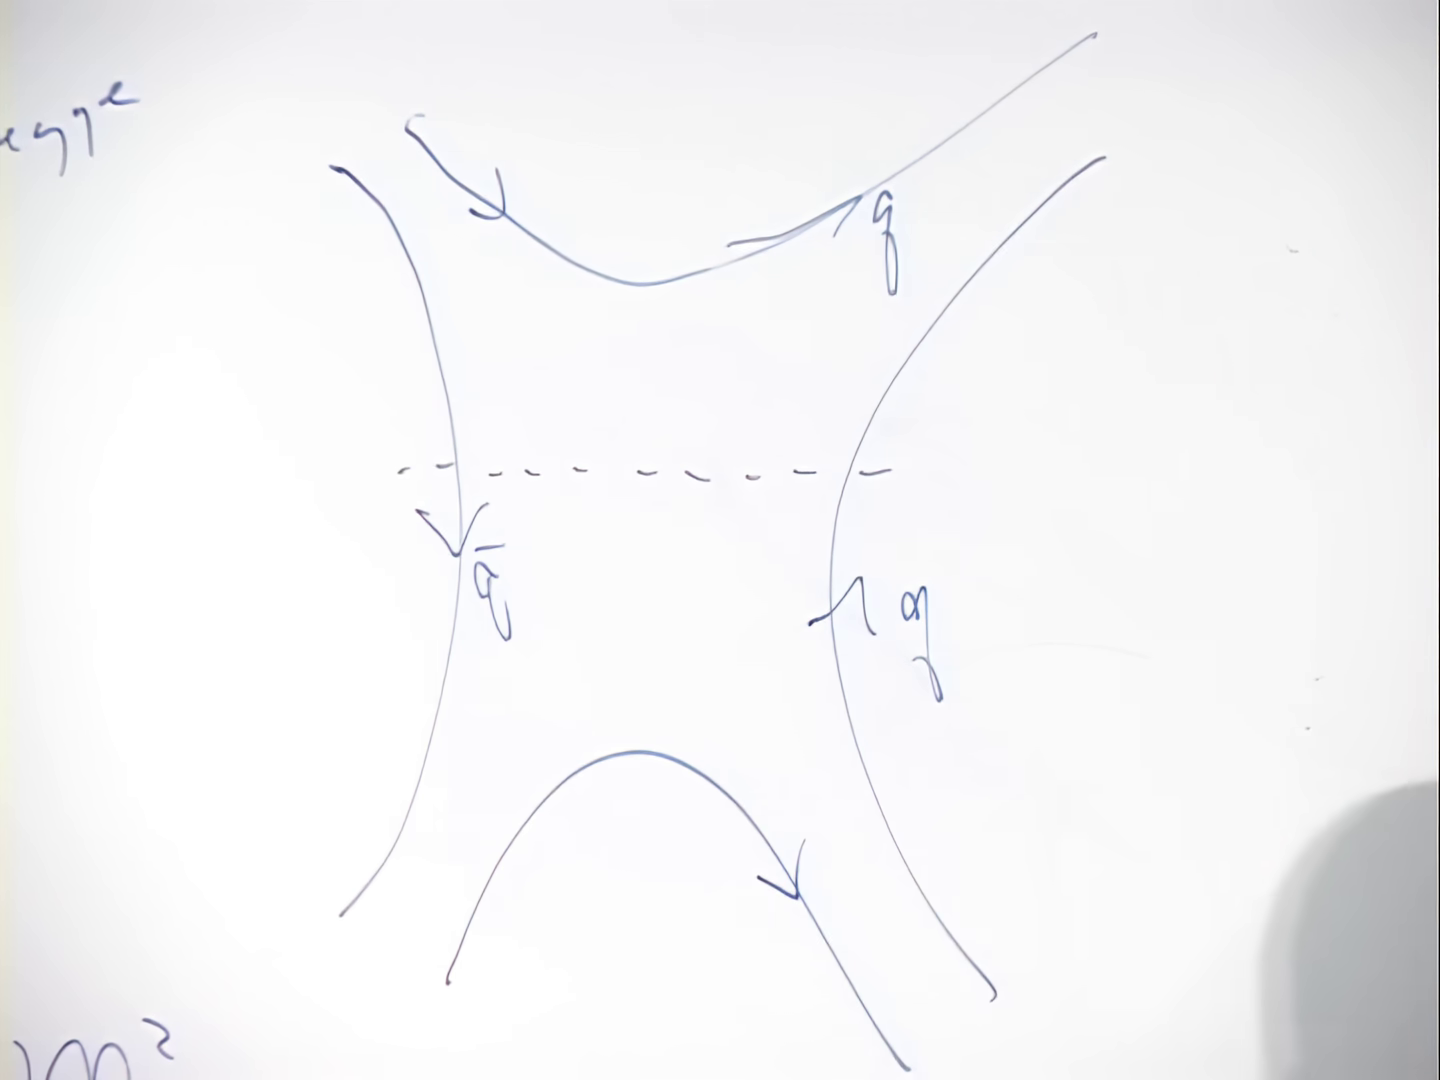
\includegraphics[width=0.78\textwidth]{lecture_01_figure_02.png}
  \caption{图上的夸克线拓扑。对同一二维历史作不同的切割，产生共振解读和交换解读。}
  \lectureframe{00:17:50}
  \label{fig:l01-worldsheet-topology-board}
\end{figure}

夸克与反夸克之间的区域提供了进一步的想法。在固定时刻，切片包含两个端点以及填满它们之间整个区间的某种东西。那个东西是一维的：一条弦。在相互作用过程中，弦扫出一个二维曲面。

\begin{definition}
点粒子的时空历史是一条\emph{世界线}。弦的时空历史是一个\emph{世界面}。某一瞬间的弦是其世界面的一个空间切片。
\end{definition}

\begin{figure}[H]
  \centering
  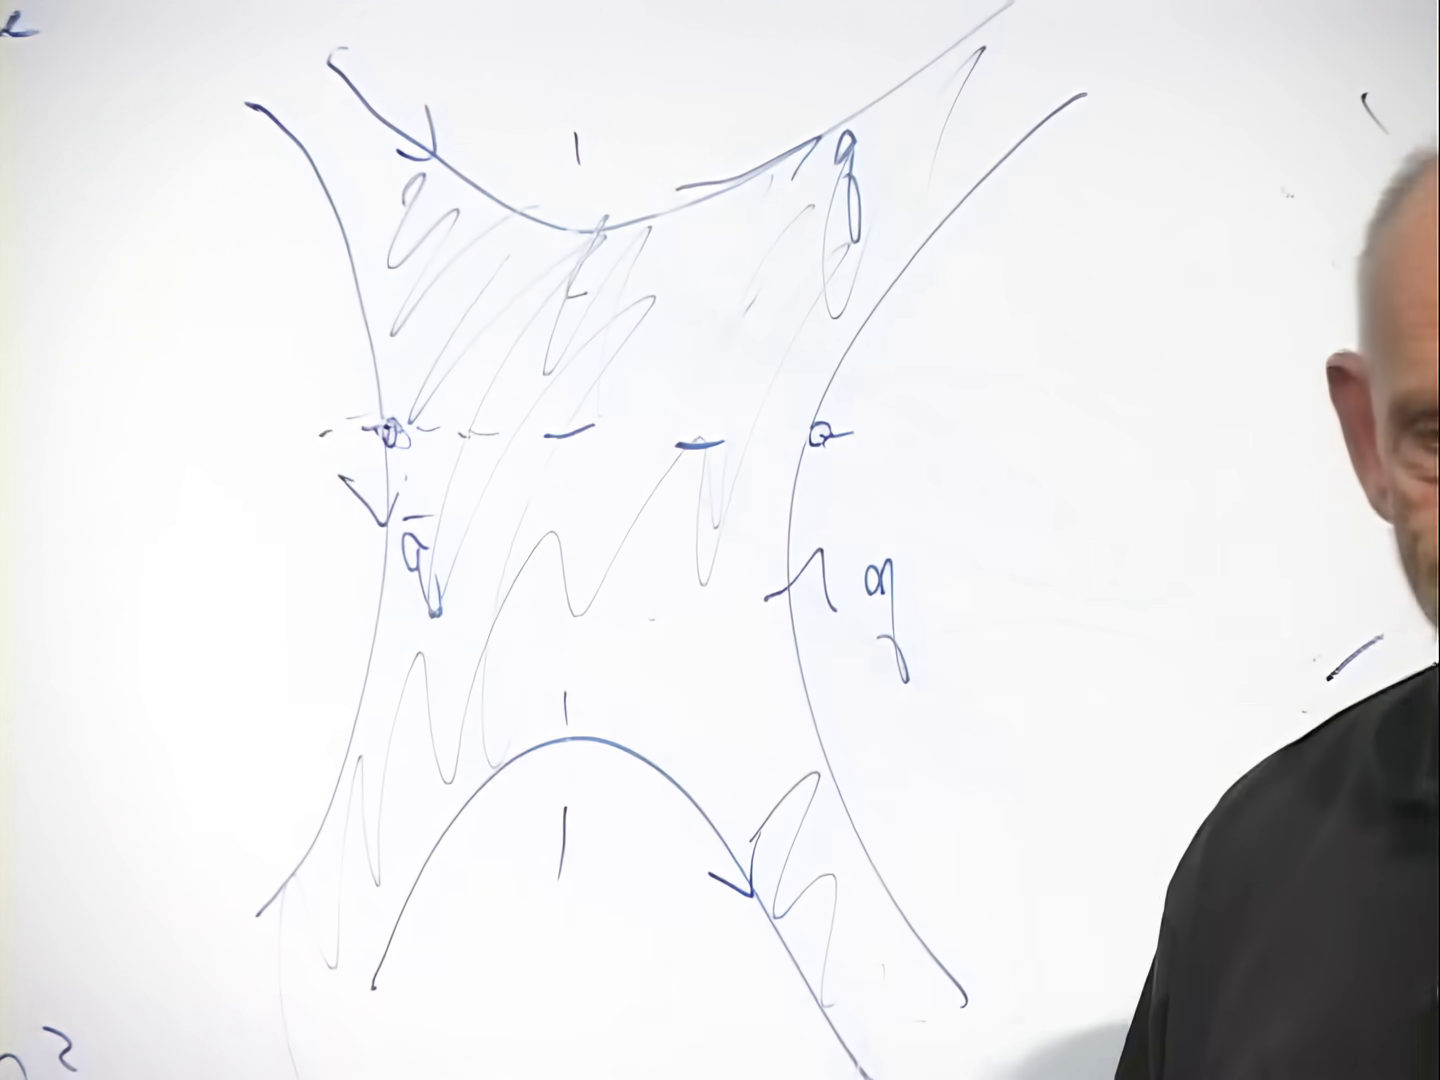
\includegraphics[width=0.78\textwidth]{lecture_01_figure_03.png}
  \caption{图上填充在端点轨迹之间的曲面。一个时间切片与它相交，得到一条一维弦。}
  \lectureframe{00:19:15}
  \label{fig:l01-worldsheet-filled-board}
\end{figure}

\begin{figure}[H]
  \centering
  \begin{tikzpicture}[>=Latex,scale=0.95]
    \fill[blue!10]
      (-2.6,-2.3) .. controls (-1.0,-1.0) and (-1.0,-0.4) .. (-0.2,0)
      .. controls (-1.0,0.5) and (-1.0,1.0) .. (-2.6,2.3)
      -- (2.6,2.3)
      .. controls (1.0,1.0) and (1.0,0.5) .. (0.2,0)
      .. controls (1.0,-0.4) and (1.0,-1.0) .. (2.6,-2.3) -- cycle;
    \draw[blue!65!black]
      (-2.6,-2.3) .. controls (-1.0,-1.0) and (-1.0,-0.4) .. (-0.2,0)
      .. controls (-1.0,0.5) and (-1.0,1.0) .. (-2.6,2.3);
    \draw[blue!65!black]
      (2.6,-2.3) .. controls (1.0,-1.0) and (1.0,-0.4) .. (0.2,0)
      .. controls (1.0,0.5) and (1.0,1.0) .. (2.6,2.3);
    \draw[red!75!black,dashed] (-2.9,-1.15) -- (2.9,-1.15)
      node[right] {time slice};
    \draw[orange!80!black,dashed] (-1.55,-2.5) -- (1.55,2.5)
      node[above] {crossed slicing};
    \draw[->] (3.45,-1.7) -- (3.45,1.8) node[above] {time};
    \node[blue!65!black] at (0,-2.7) {one world sheet};
  \end{tikzpicture}
  \caption{一个清晰的世界面示意图。不同的切片方式把同一个曲面组织成不同的中间道描述。}
  \label{fig:l01-worldsheet-redraw}
\end{figure}

这种几何重构是探索性的，并不是从第一性原理推导出完整理论。不同的人以不同方式达到了早期的弦图像。它的力量在于，同一个延展物体可以同时处理这两种观测：弦可以旋转和形变，而它的世界面可以编码对偶的散射道。

\begin{classroomqa}
\audiencequestion{为什么要引入一个弦状的桥梁，而不是在夸克之间交换一个普通粒子？\lecturetimestamp{00:21:20}}
\lecturerresponse{在某一瞬间，不仅仅存在一个局域化的交换粒子。存在一个夸克、一个反夸克，以及它们之间所有点处的结构。这种结构可能是基本连续的，也可能是大量组分密集聚集而近似为连续体；第一种图像并未作出判定。重要的是整个区间都被占据，而且观测到的轨迹没有表现出像两端系着重物的普通鞋带那样终止的倾向。}
\end{classroomqa}

\begin{classroomqa}
\audiencequestion{标准模型能描述{\proseunicodefont π}介子散射吗？
\lecturetimestamp{00:22:45}}
\lecturerresponse{能，尽管其有用性取决于能区。在低能下，标准模型通过QCD及其低能描述，能够解释大量的{\proseunicodefont π}介子散射。在较高能量下，当整族的强子交换都变得重要时，直接计算变得更加困难，而弦式的组织方式可能更为有用。}
\end{classroomqa}

\begin{classroomqa}
\audiencequestion{早期实验是否确立了Regge轨迹永不终止？\lecturetimestamp{00:23:37}}
\lecturerresponse{没有。它们只确立了所观测到的序列尚未显示出终点。关于可无限延伸的推断是一种富有启发性的外推，而不是被测量到的无限。}
\end{classroomqa}

\section{通量管与标度的变化}

现代QCD为这一旧图像提供了场论解释。夸克与反夸克充当胶子场的相反源。在普通电动力学中，当相反电荷被分开时，电通量会向侧面扩展。场随距离减弱，因此电荷之间的区域不会保持固定的横向剖面。QCD是非线性的。其动力学可以将相关的色电场通量限制在连接夸克与反夸克的狭窄管中。

\begin{figure}[H]
  \centering
  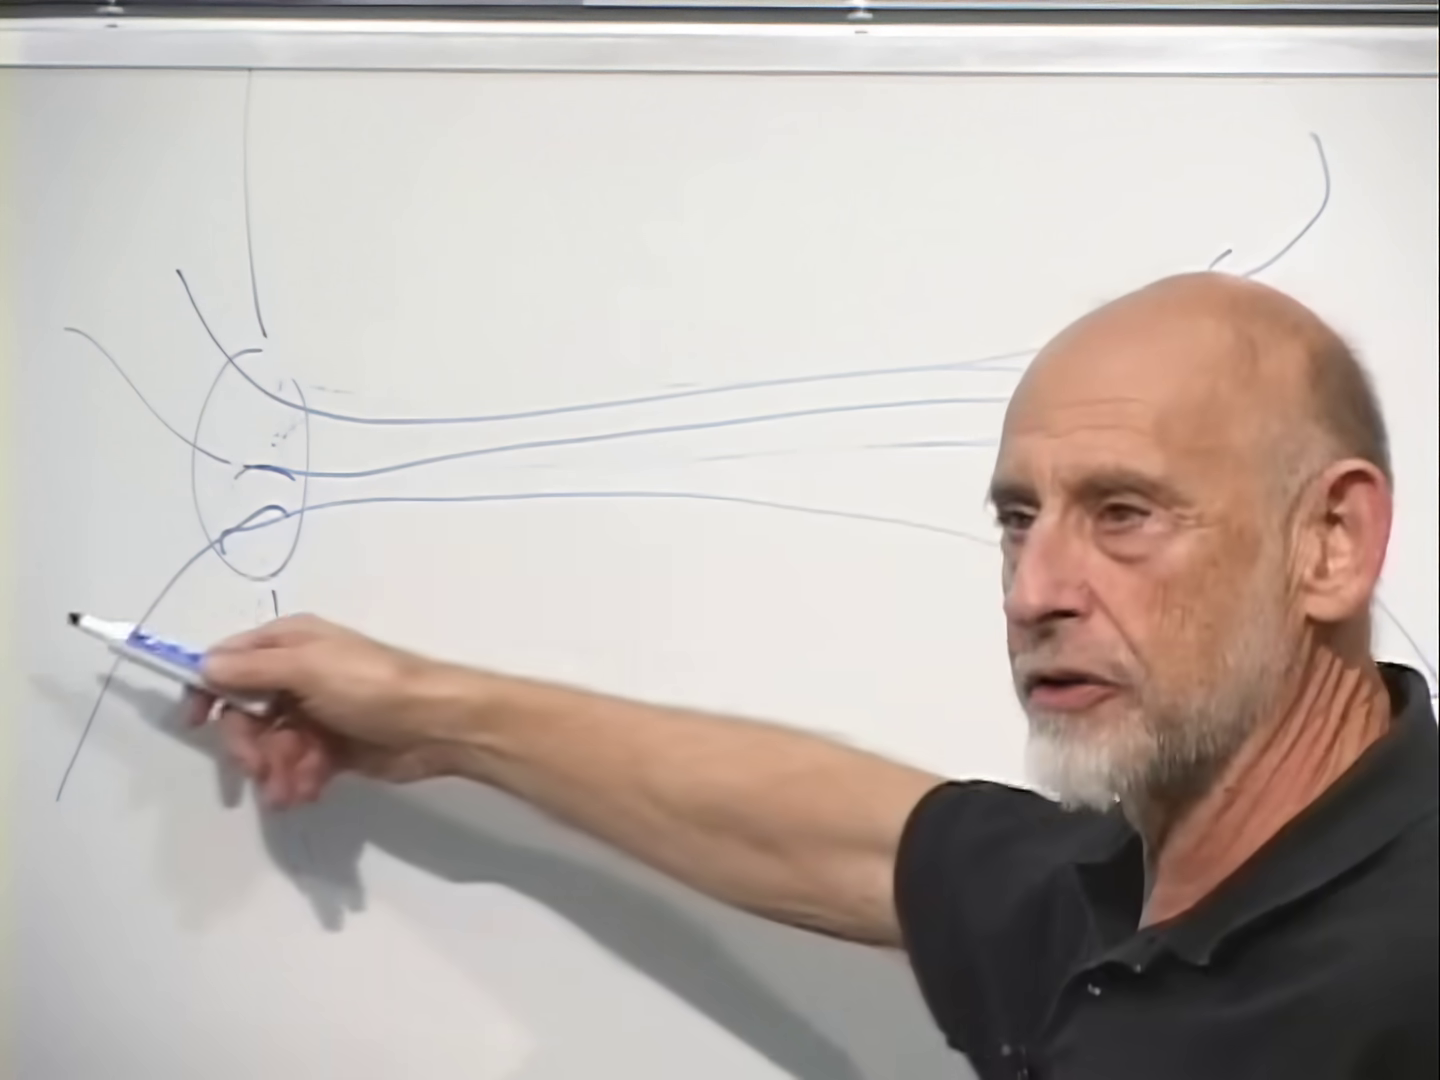
\includegraphics[width=0.78\textwidth]{lecture_01_figure_04.png}
  \caption{夸克与反夸克的场线被画成狭窄的通量管，而不是自由扩展的库仑场。}
  \lectureframe{00:25:15}
  \label{fig:l01-qcd-flux-board}
\end{figure}

\begin{figure}[H]
  \centering
  \begin{tikzpicture}[>=Latex]
    \fill[orange!14,rounded corners=8pt] (-3.0,-0.55) rectangle (3.0,0.55);
    \draw[orange!80!black,thick,rounded corners=8pt]
      (-3.0,-0.55) rectangle (3.0,0.55);
    \fill[blue!70!black] (-3.35,0) circle (0.17);
    \fill[red!75!black] (3.35,0) circle (0.17);
    \node[below] at (-3.35,-0.22) {$q$};
    \node[below] at (3.35,-0.22) {$\bar q$};
    \foreach \y in {-0.30,0,0.30}
      \draw[->,orange!85!black] (-3.05,\y) -- (3.05,\y);
    \draw[<->] (-2.9,-1.05) -- (2.9,-1.05) node[midway,below] {$L$};
    \node at (0,0.92) {approximately fixed transverse profile};
  \end{tikzpicture}
  \caption{被禁闭的通量管在伸长时不扩展。固定的单位长度能量给出\(E=TL\)。}
  \label{fig:l01-qcd-flux-redraw}
\end{figure}

粒子语言与场语言以不同方式表达同一件事。在场描述中，当两端分离时，管保持大致相同的场强和横截面积。在组分图像中，拉伸能量在两端之间产生更多的胶子结构。普通橡皮筋具有固定数目的分子，因此其分子会彼此分离，直到材料断裂。不妨设想，每当出现一个空隙时就插入一个新分子。这样，沿带的密度可以保持固定，而带却变得更长。这就是对胶子场的预期类比：管获得长度，而不是变细直至断裂。

\begin{classroomqa}
\audiencequestion{构成电子的弦是否也会由胶子组成？\lecturetimestamp{00:28:08}}
\lecturerresponse{得不出这样的结论。强子弦是质子尺度上的QCD客体。与量子引力相关的假想基本弦将位于小得多的普朗克尺度附近，而这里没有证据表明电子是强子胶子弦。引人注目的事实是，相关的数学在两个尺度上都出现了，而不是物理客体本身相同。}
\end{classroomqa}

将强子图像转变为完整的相互作用弦理论的尝试很有前景，但并未完全产生所期望的强子理论。该数学模型一再包含一个自旋为二的无质量粒子。在强子理论中，该态看起来像是一个不受欢迎的预言；而作为引力理论，它具有的量子数恰好就是引力子的量子数。Joel Scherk和John Schwarz作出了决定性的重新解释：也许这个理论告诉我们的不是强子，而是量子引力。强子应用与基本应用在物理上是不同的，尽管早期的强子问题提供了通向这一数学的路径。

\begin{classroomqa}
\audiencequestion{通量线如何从正端点走向负端点？\lecturetimestamp{00:31:46}}
\lecturerresponse{它们离开一个源并进入另一个源，正如磁力线从条形磁铁的北极延伸到南极。相反的端点标记表达了通量的取向；条形磁铁同样具有两个相反的磁极，而不是两个北极。}
\end{classroomqa}

\begin{classroomqa}
\audiencequestion{弦是连续的还是离散的？
\lecturetimestamp{00:32:45}}
\lecturerresponse{量子理论使这一区分变得微妙。电磁场被表示为连续场，同时也具有离散的量子。同样，弦可以被连续地处理，而其激发是量子化的。两种描述都可以是有效的，取决于所提出的问题。}
\end{classroomqa}

\begin{classroomqa}
\audiencequestion{如果穿过世界面的时空切片的角度发生改变，其交线仍然是一条弦吗？\lecturetimestamp{00:34:20}}
\lecturerresponse{是的。改变同时性切片是一种洛伦兹变换。新的切片与该曲面相交所得的弦，处于不同的运动状态。即使一条弦的质心处于静止，其内部也并非静止不动；它可能在振动。``静止''仅指其质心而言。}
\end{classroomqa}

\section{相对论能量的两种展开}

对延展的振动客体作直接的相对论描述颇为不便。有用的策略是找到一个参考系，使其相关运动具有普通非相对论力学的形式。先从单个粒子开始。非相对论情形下可写为

\begin{equation}
  E_{\mathrm{nr}}=\frac{\bm p^2}{2m}+B,
  \label{eq:l01-nonrel-energy}
\end{equation}

其中\(B\)是与总动量无关的内能或束缚能。对于多个无相互作用的粒子，动能项与内能常数项分别相加。由于只有能量差决定运动，与状态无关的相加常数往往可以略去。

精确的相对论能量为

\begin{equation}
  E=\sqrt{\bm p^2c^2+m^2c^4}.
  \label{eq:l01-rel-energy-c}
\end{equation}

\begin{figure}[H]
  \centering
  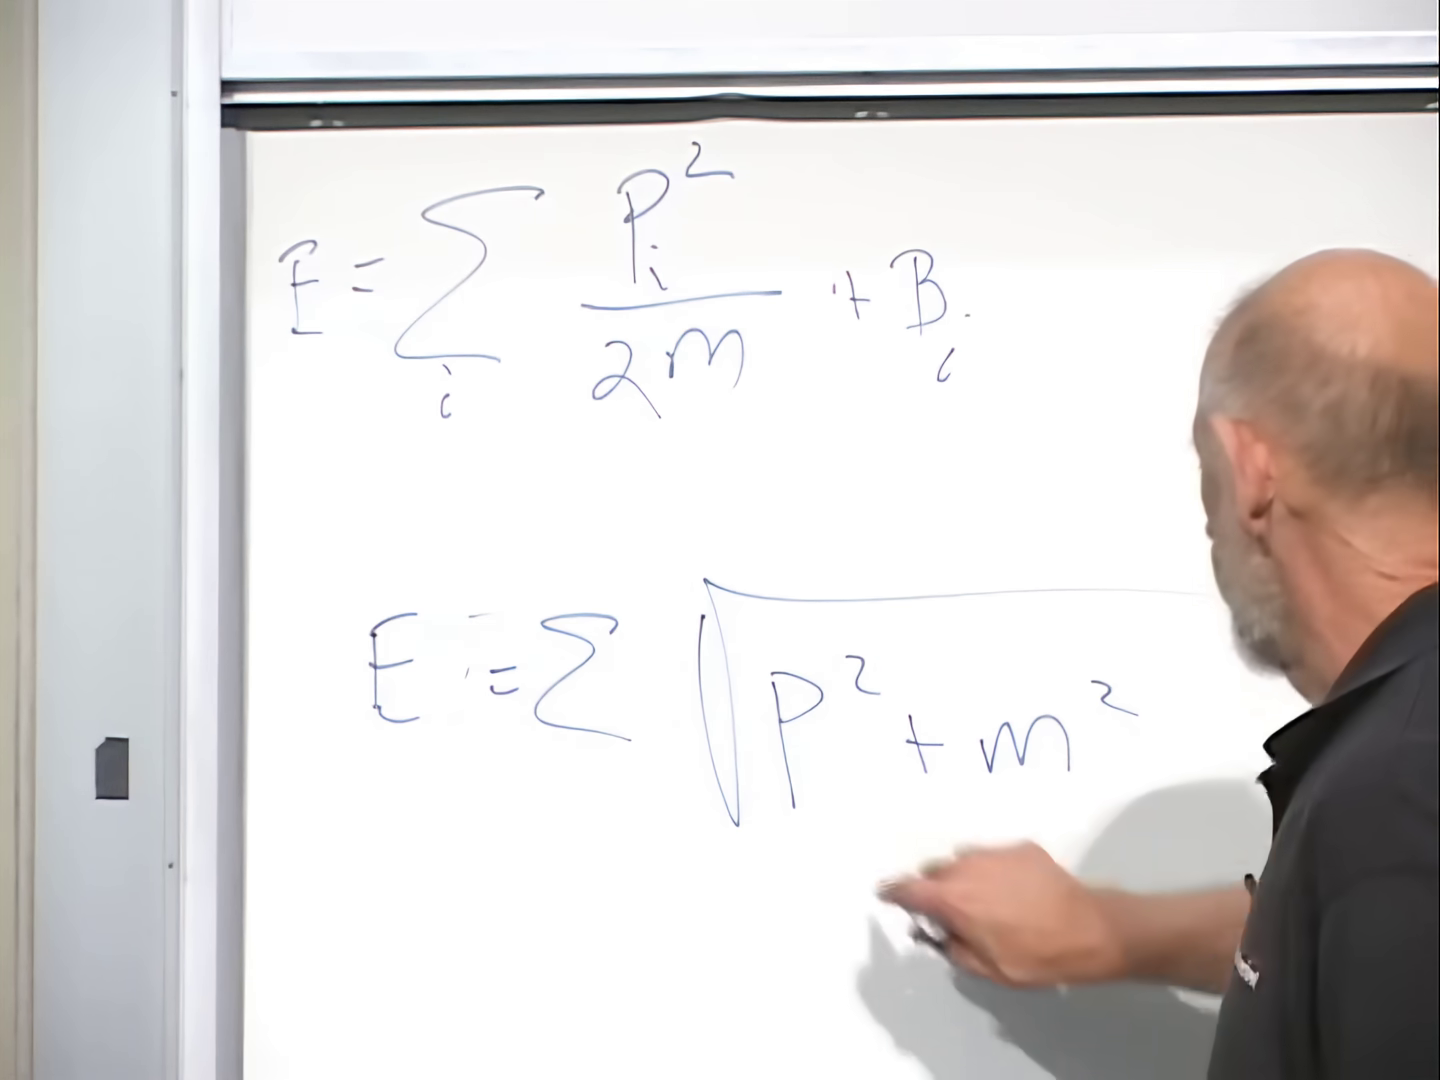
\includegraphics[width=0.76\textwidth]{lecture_01_figure_05.png}
  \caption{非相对论动能与精确的相对论平方根，讨论中已修正\(c\)的幂次。}
  \lectureframe{00:38:45}
  \label{fig:l01-relativistic-energy-board}
\end{figure}

\begin{classroomqa}
\audiencequestion{相对论公式中是否应包含\(p^2c^2\)和
\(m^2c^4\)，而不是最初写在黑板上的那些幂次？
\lecturetimestamp{00:39:12}}
\lecturerresponse{是的。量纲一致性将表达式确定为
\(E^2=p^2c^2+m^2c^4\)。在恢复非相对论极限之后，我们将取
\(c=1\)，但在此处保留这些幂次可使展开更为清晰。}
\end{classroomqa}

当\(p^2c^2\ll m^2c^4\)时，提出\(m^2c^4\)并利用
\(\sqrt{1+\epsilon}\simeq1+\epsilon/2\)：

\begin{align}
  E
  &=mc^2\sqrt{1+\frac{p^2}{m^2c^2}}
  \notag\\
  &\simeq mc^2+\frac{p^2}{2m}.
  \label{eq:l01-low-momentum-expansion}
\end{align}

\begin{figure}[H]
  \centering
  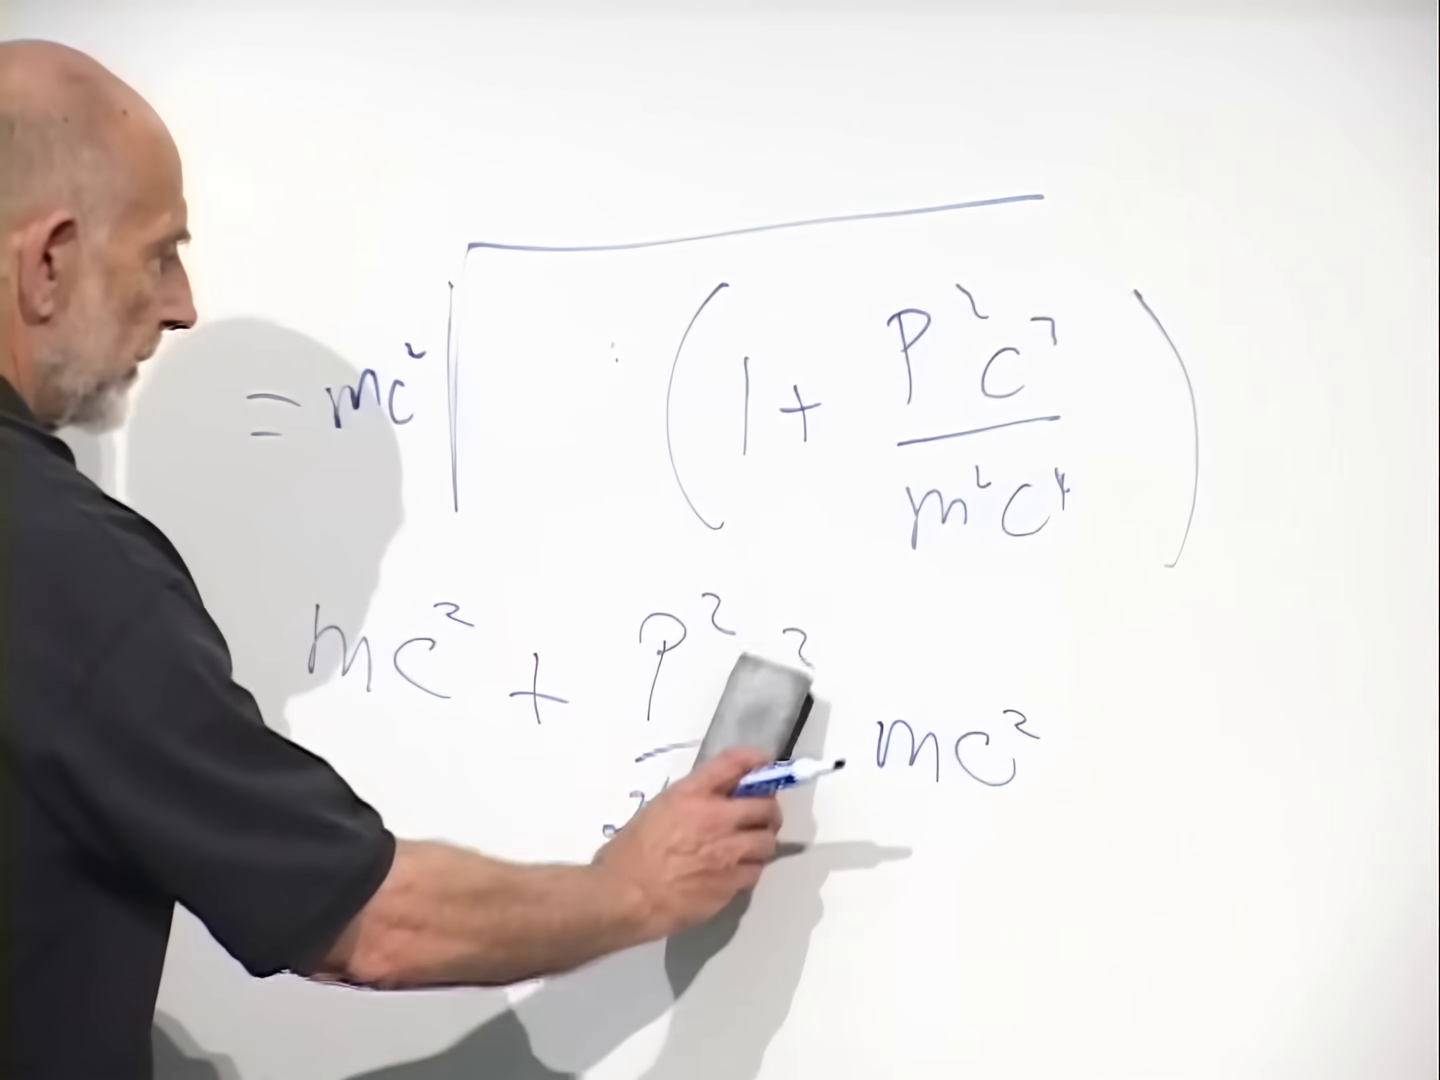
\includegraphics[width=0.76\textwidth]{lecture_01_figure_06.png}
  \caption{小动量展开，恢复出静止能量加上熟悉的非相对论动能项。}
  \lectureframe{00:41:30}
  \label{fig:l01-low-momentum-board}
\end{figure}

这一近似所要求的不仅仅是质心的缓慢运动。一个盒子可以缓慢漂移，而其中的粒子却以接近光速运动。在这种情况下，内部动力学仍然是相对论的。普通的非相对论极限要求所有相关组成粒子的速度在所选参考系中都很小。

还有另一种有用的极限。将整个系统沿\(z\)轴加速，直到每个组成粒子都具有很大的正纵向动量\(P_{zi}\)。任何最初向后运动的组成粒子都会被足够大的加速带到前方。横向动量和静止质量保持不变：

\begin{equation}
  P_{zi}\gg |p_{xi}|,|p_{yi}|,m_i,
  \qquad
  p_{\perp i}^2=p_{xi}^2+p_{yi}^2,
\end{equation}

其中从此刻起\(c=1\)。对大的\(P_{zi}\)作展开得到

\begin{align}
  E_i
  &=\sqrt{P_{zi}^2+p_{\perp i}^2+m_i^2}
  \notag\\
  &=P_{zi}\sqrt{1+\frac{p_{\perp i}^2+m_i^2}{P_{zi}^2}}
  \notag\\
  &\simeq P_{zi}
  +\frac{p_{\perp i}^2+m_i^2}{2P_{zi}}.
  \label{eq:l01-large-pz-one-particle}
\end{align}

\begin{figure}[H]
  \centering
  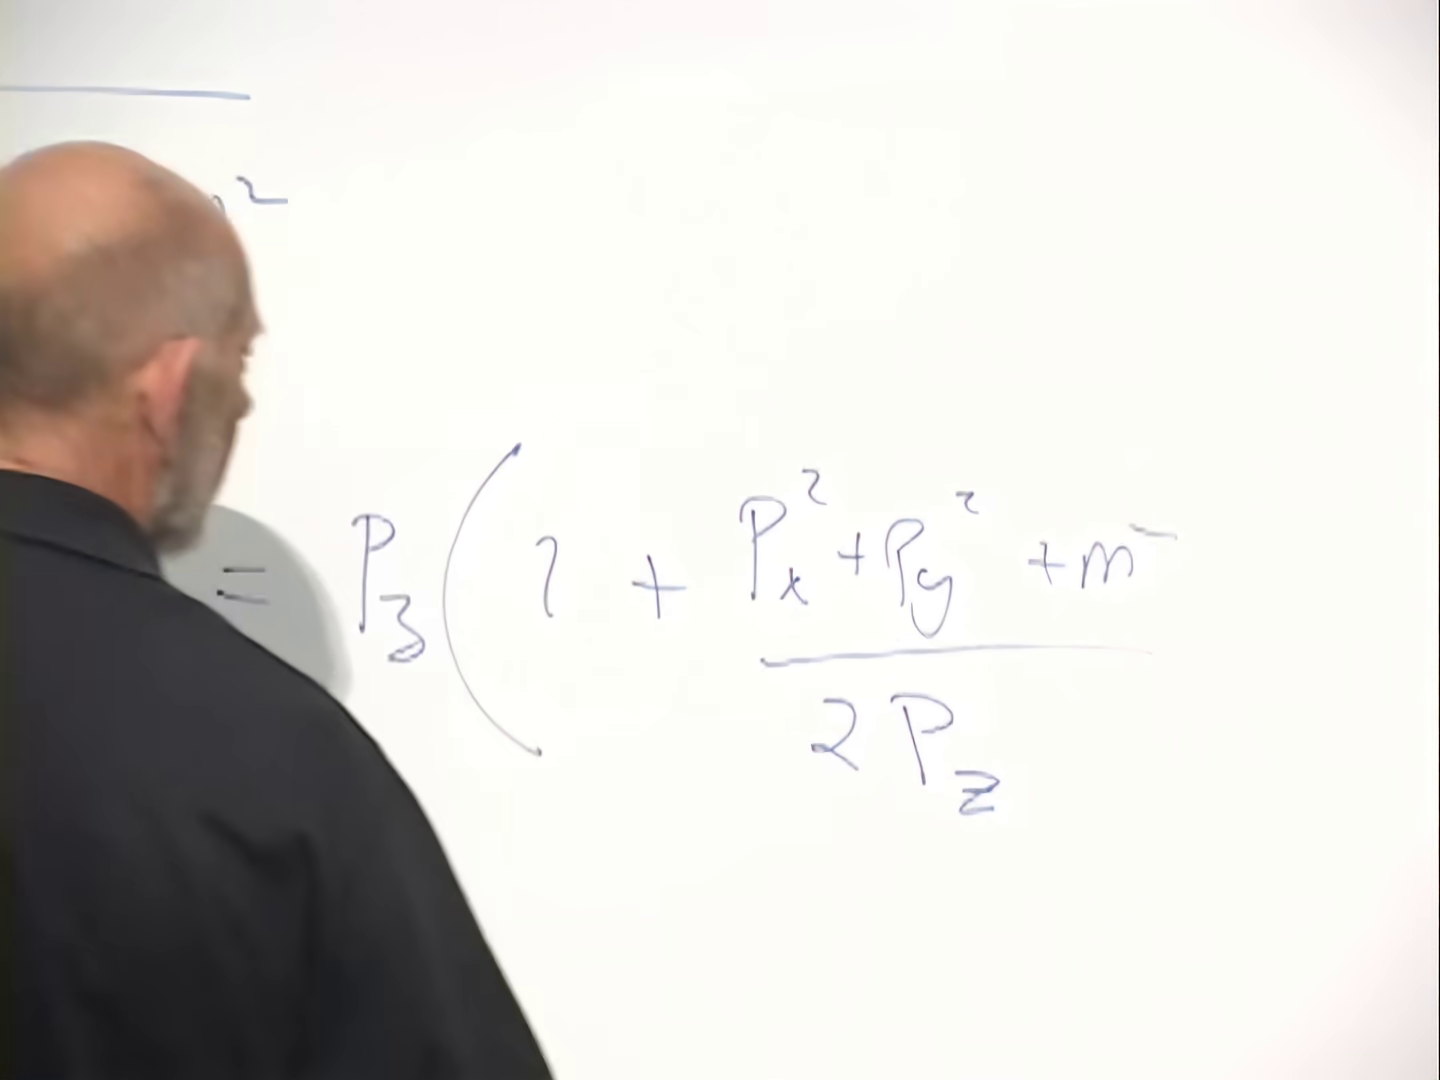
\includegraphics[width=0.76\textwidth]{lecture_01_figure_07.png}
  \caption{大\(P_z\)下的平方根展开，横向动量和质量作为小量保留。}
  \lectureframe{00:46:45}
  \label{fig:l01-large-pz-board}
\end{figure}

对于多个组成粒子，

\begin{equation}
  E\simeq
  \sum_i P_{zi}
  +\sum_i\frac{p_{\perp i}^2}{2P_{zi}}
  +\sum_i\frac{m_i^2}{2P_{zi}}.
  \label{eq:l01-large-pz-sum}
\end{equation}

第一项是守恒的总纵向动量。它极其巨大，但也是一个固定的相加贡献。保留它或减去它都不会改变任何能量差，正如在哈密顿量中加上任何其他守恒量都不会改变运动方程一样。因此动力学部分为

\begin{equation}
  \begin{aligned}
    H_{\perp}=E-P_z
    &\simeq
    \sum_i\left(
      \frac{p_{\perp i}^2}{2P_{zi}}
      +\frac{m_i^2}{2P_{zi}}
    \right),\\
    P_z&=\sum_iP_{zi}.
  \end{aligned}
  \label{eq:l01-transverse-hamiltonian}
\end{equation}

\begin{figure}[H]
  \centering
  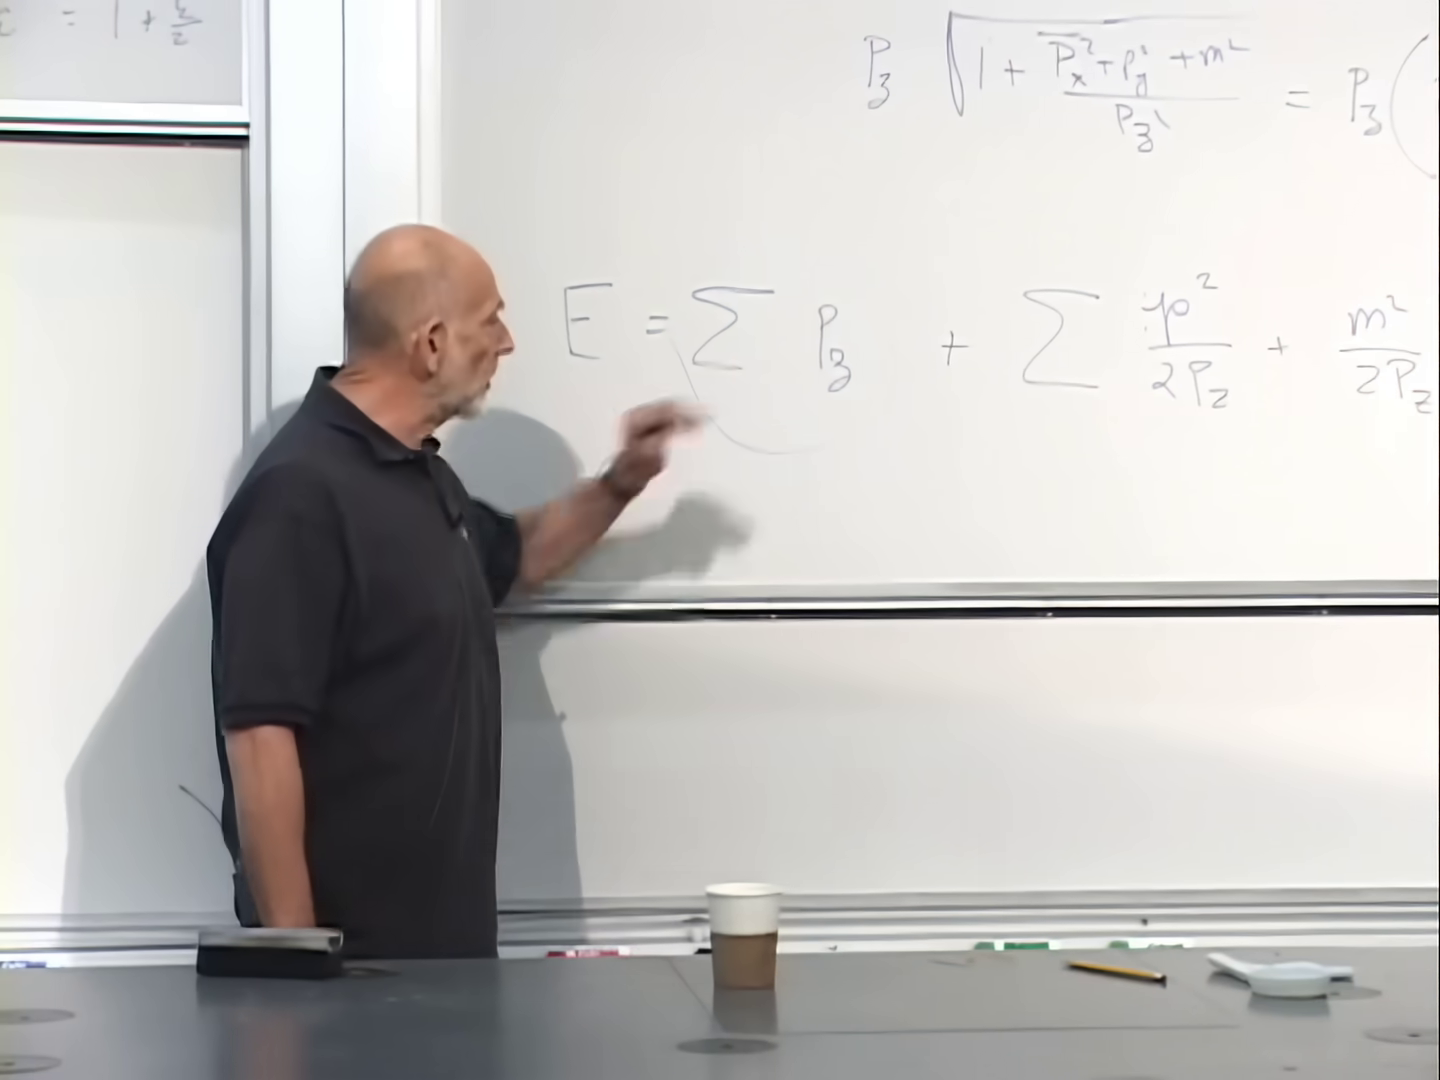
\includegraphics[width=0.78\textwidth]{lecture_01_figure_08.png}
  \caption{多粒子分解为守恒的纵向动量、横向动能以及依赖于质量的内部项。}
  \lectureframe{00:49:16}
  \label{fig:l01-energy-sum-board}
\end{figure}

\section{无限动量参考系}

上述极限在历史上被称为无限动量参考系，现在通常用光锥坐标来表述。其含义可以直接从哈密顿量读出。在量子力学中，

\begin{equation}
  i\hbar\frac{\partial}{\partial t}\ket{\psi}=H\ket{\psi}.
  \label{eq:l01-time-evolution}
\end{equation}

\(H_{\perp}\)中所有非平凡项都按\(1/P_z\)标度。随着加速增大，能量分裂缩小，变化发生得更慢。这就是时间膨胀。一个放射性系统在被高度加速时似乎衰变得更慢；人们可以通过按比例延长观测时间来补偿。这种减慢并未消除动力学。它只是重新标度了它们的时钟。

\begin{figure}[H]
  \centering
  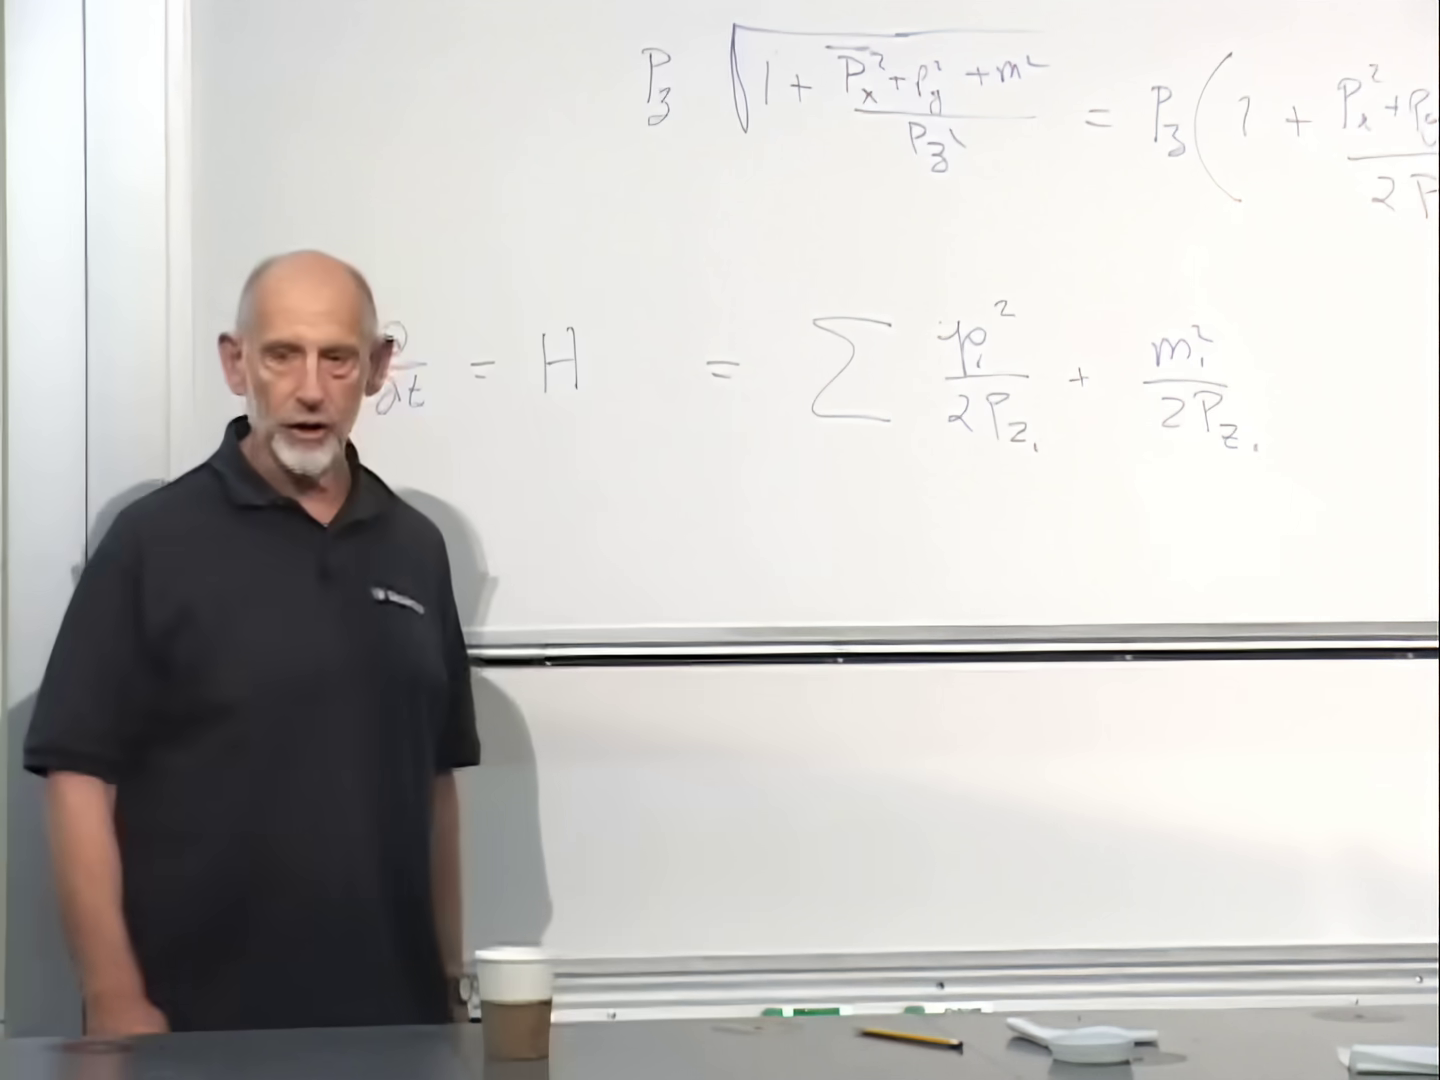
\includegraphics[width=0.78\textwidth]{lecture_01_figure_09.png}
  \caption{黑板上将约化能量等同于产生被加速系统减慢的时间演化的哈密顿量。}
  \lectureframe{00:52:57}
  \label{fig:l01-hamiltonian-board}
\end{figure}

横向项具有精确的非相对论形式 \(p^2/(2m)\)，但质量的角色由 \(P_z\) 扮演。这在物理上是合理的：更大的纵向动量使粒子更难被横向偏转，因此它起到横向惯性的作用。\(m_i^2/(2P_{zi})\) 项不依赖于二维运动状态，因此扮演内能或束缚能的角色。三个空间维度中的相对论运动已变成垂直于推进方向的两个维度中看似非相对论的运动。

这正是使用相对论弦的基本质量-弹簧模型所需的许可。该模型并非假装弦在其静止系中运动缓慢。它使用的是横向动力学具有所需非相对论结构的参考系。

\section{由珠子和弹簧构成的开弦}

取一根开弦，即具有两个端点的弦。之后可能有东西附着在这些端点上，但当前关注的是弦本身。用位于横向位置 \(\bm X_i(t)=(X_i(t),Y_i(t))\) 的珠子来近似它，珠子之间由相同的弹簧连接。离散哈密顿量为

\begin{equation}
  H_N=\sum_{i=1}^{N}
  \left[
    \frac{\mu_N}{2}\dot{\bm X}_i^{\,2}
    +\frac{k_N}{2}
      \left(\bm X_{i+1}-\bm X_i\right)^2
  \right].
  \label{eq:l01-discrete-string}
\end{equation}

仅动能项会使珠子飞散开来。最近邻胡克项才使它们成为一根弦。

\begin{figure}[H]
  \centering
  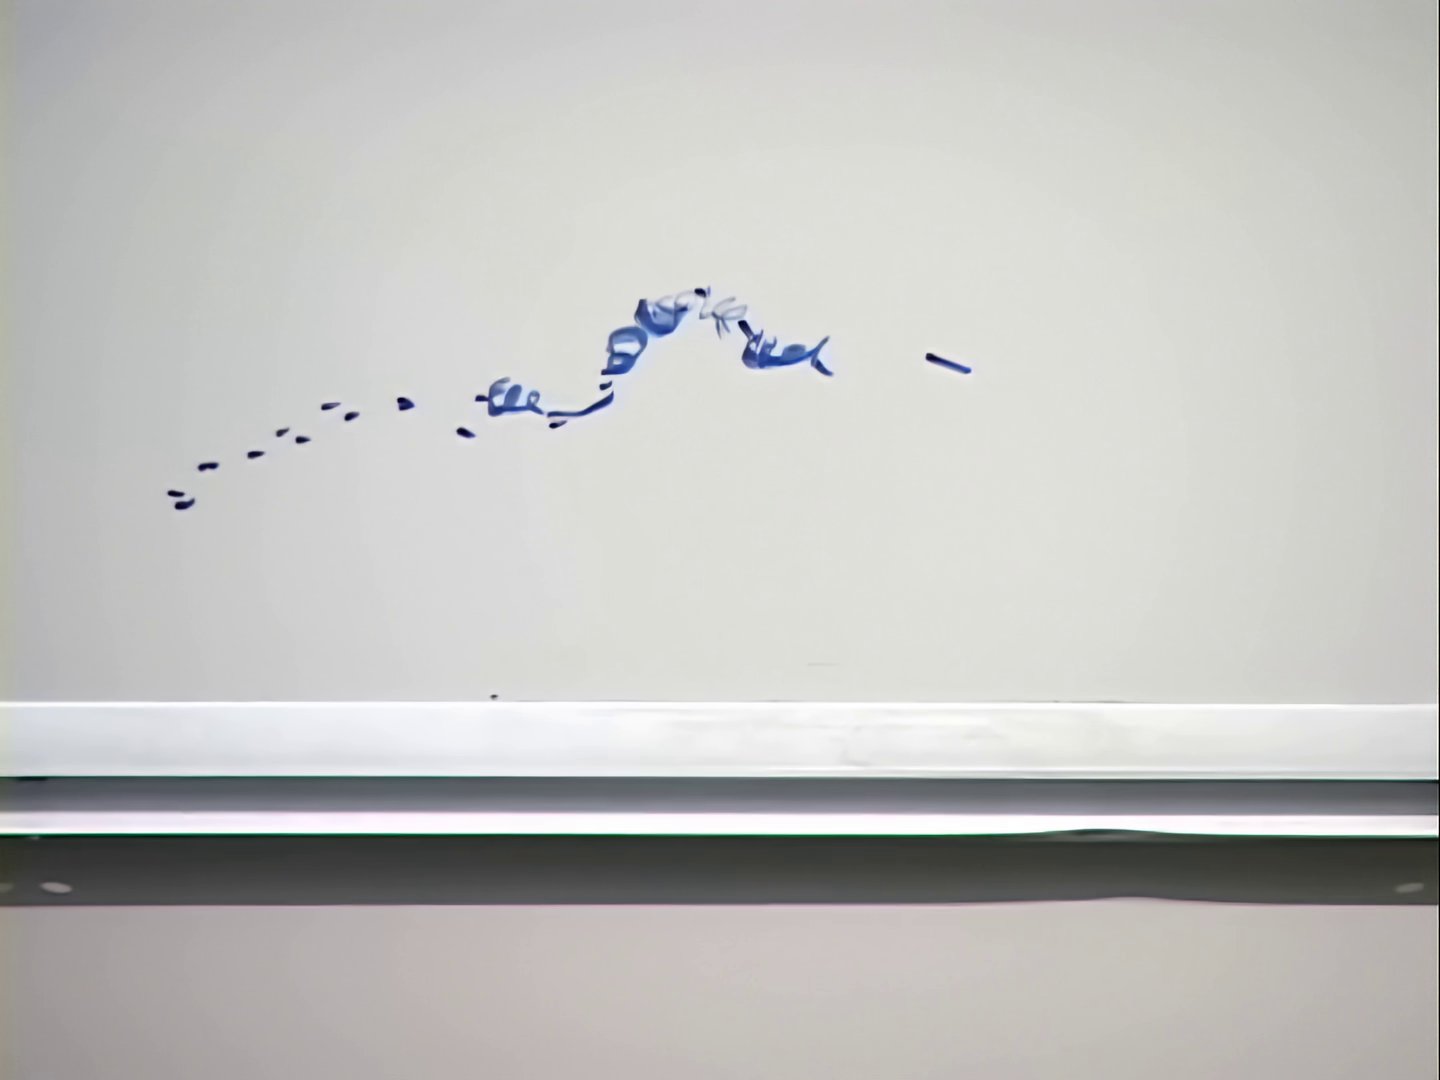
\includegraphics[width=0.75\textwidth]{lecture_01_figure_10.png}
  \caption{具有两个横向坐标的开弦的第一幅珠子-弹簧示意图。}
  \lectureframe{01:00:30}
  \label{fig:l01-bead-chain-board}
\end{figure}

\begin{figure}[H]
  \centering
  \begin{tikzpicture}[>=Latex]
    \foreach \x in {0,...,8} {
      \fill[blue!65!black] ({0.85*\x},0) circle (0.09);
    }
    \foreach \x in {0,...,7} {
      \draw[decorate,decoration={zigzag,segment length=4pt,amplitude=2pt}]
        ({0.85*\x+0.10},0) -- ({0.85*\x+0.75},0);
    }
    \draw[->] (3.4,0.15) -- (3.4,1.25) node[above] {$\bm X_i(t)$};
    \draw[<->] (0,-0.65) -- (6.8,-0.65)
      node[midway,below] {$0\leq\sigma\leq\pi$};
  \end{tikzpicture}
  \caption{开弦的离散正规化。在取连续极限之前，珠子质量和弹簧常数随间距缩放。}
  \label{fig:l01-bead-chain-redraw}
\end{figure}

\begin{figure}[H]
  \centering
  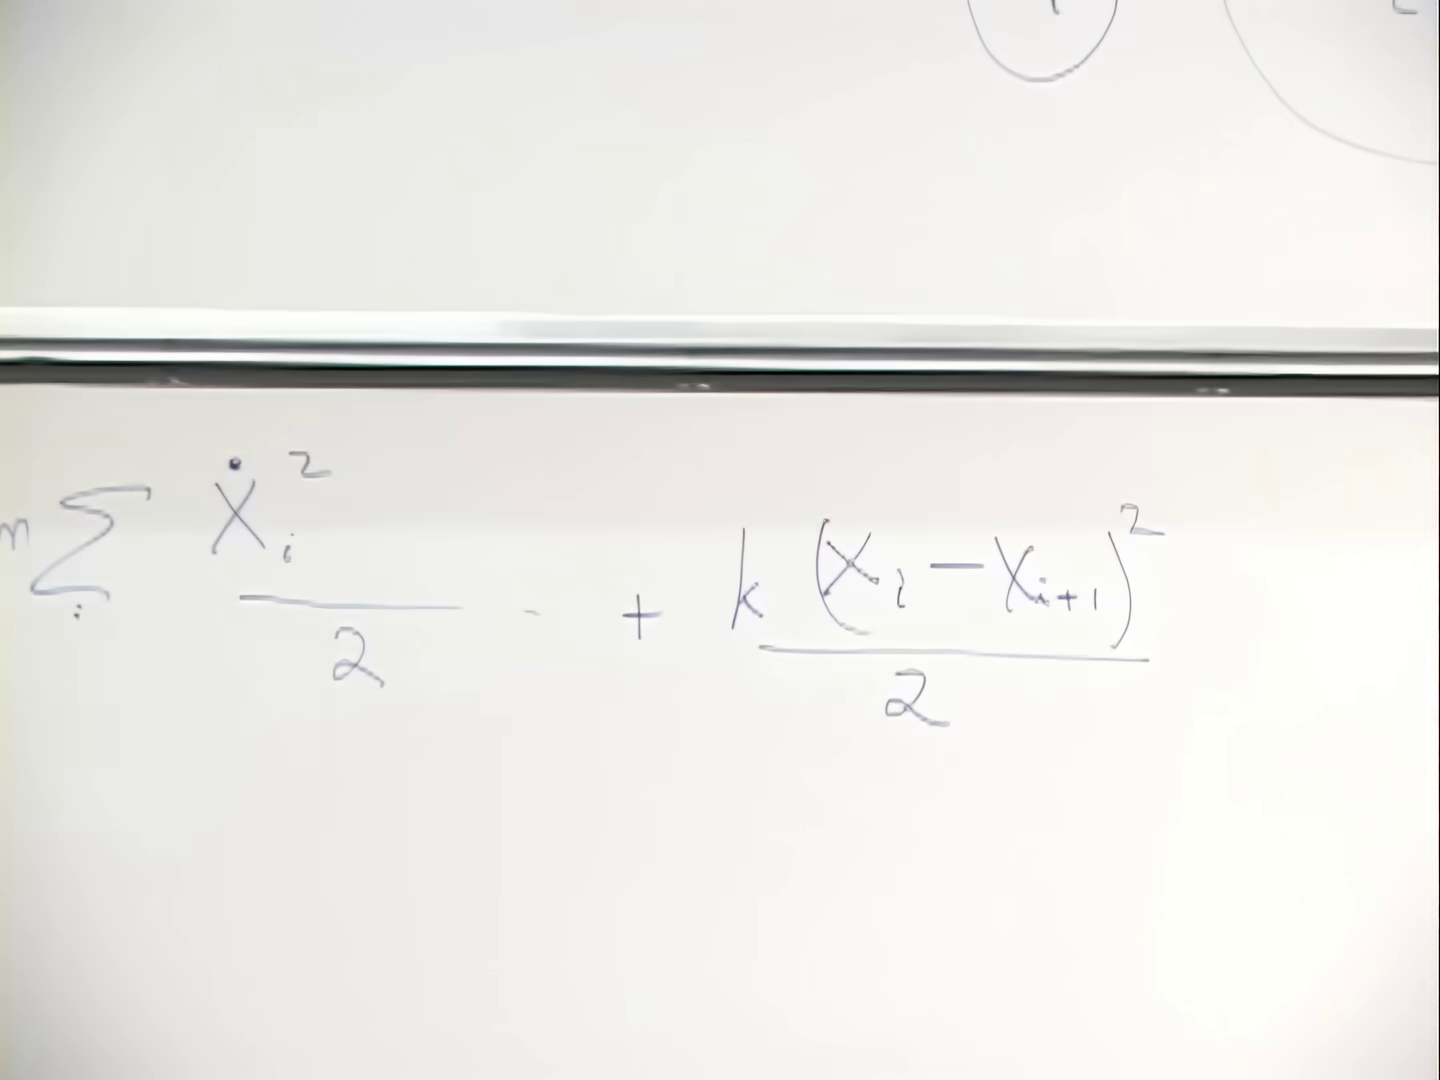
\includegraphics[width=0.78\textwidth]{lecture_01_figure_11.png}
  \caption{在取连续极限之前写在一起的离散动能项和胡克项。}
  \lectureframe{01:01:30}
  \label{fig:l01-discrete-energy-board}
\end{figure}

随着珠子数目的增加，每个珠子的质量 \(\mu_N\) 必须趋于零，以使整根弦保持有限的惯性。与此同时，弹簧常数 \(k_N\) 必须增大。一条长橡胶带比同种材料的一小段更容易被拉伸固定量；因此，如果连续材料要保持相同，被拉得更近的相邻点必须以更大的劲度相连。

引入沿弦的坐标 \(\sigma\)。其数值范围是一种约定。选择

\begin{equation}
  0\leq\sigma\leq\pi
\end{equation}

是方便的，因为闭弦之后可以从 \(0\) 参数化到 \(2\pi\)。求和变为积分，最近邻差分变为导数：

\begin{equation}
  \sum_i\longrightarrow\int_0^\pi d\sigma,
  \qquad
  \bm X_{i+1}-\bm X_i
  \longrightarrow
  \partial_\sigma\bm X.
  \label{eq:l01-continuum-replacements}
\end{equation}

在将依赖于间距的常数吸收进 \(t\)、\(\sigma\) 和 \(\bm X\) 的归一化之后，连续哈密顿量具有如下形式

\begin{equation}
  H_{\mathrm{string}}=
  \frac12\int_0^\pi d\sigma
  \left[
    \left(\partial_t\bm X\right)^2
    +\left(\partial_\sigma\bm X\right)^2
  \right].
  \label{eq:l01-continuum-hamiltonian}
\end{equation}

\begin{figure}[H]
  \centering
  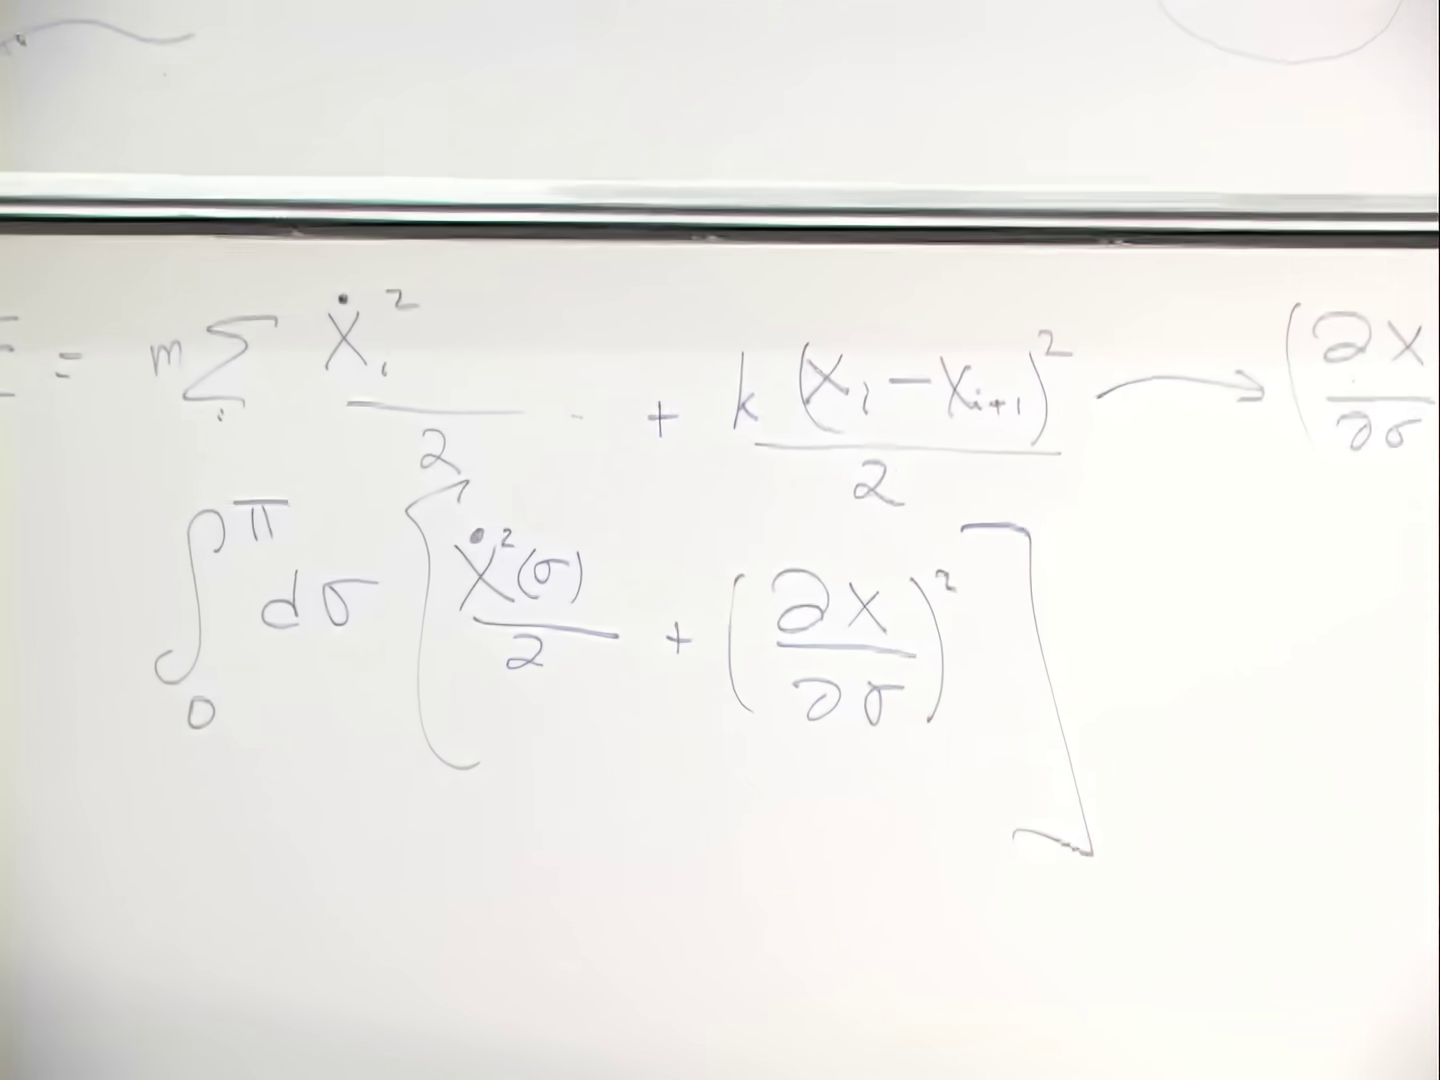
\includegraphics[width=0.78\textwidth]{lecture_01_figure_12.png}
  \caption{从珠子求和到 \(\int_0^\pi d\sigma\) 的板书推导过程，其中最近邻差分被替换为 \(\partial_\sigma\bm X\)。}
  \lectureframe{01:05:00}
  \label{fig:l01-continuum-board}
\end{figure}

第一项是两个横向方向上的动能。第二项度量沿弦的拉伸。两项都带正号，因为这是哈密顿量。在拉格朗日量中，势能项会以负号出现。精确的系数取决于约定，在此阶段尚未固定；真正重要的是动能加拉伸的结构。

将质心运动与相对运动分开。将每个点平移相同的量会使粒子整体移动。振荡、弯曲和相对拉伸是内部运动。质子、原子或任何其他复合物体都可以被称为粒子，即使其组分在内部运动。弦在这方面并无不同。

\section{为什么哈密顿量度量的是质量平方}

对于缓慢运动的物体，静能与其质量成正比。然而，在无穷动量描述中，内部贡献表现为 \(M^2/(2P_z)\)。一旦共同的纵向动量及其相关的时间重标度被固定，内部弦哈密顿量就与整个物体的不变质量平方成正比：

\begin{equation}
  H_{\mathrm{int}}\propto M^2.
  \label{eq:l01-hint-mass-squared}
\end{equation}

\editorialnote{更明确地说，光锥运动学给出形式为 \(M^2=2P^+P^- - \bm P_\perp^2\) 的不变关系。在质心横向参考系中且 \(P^+\) 固定时，光锥哈密顿量 \(P^-\) 因此与 \(M^2\) 成正比。本讲省略了这些归一化细节，只保留论证所需的比例关系。}

\begin{figure}[H]
  \centering
  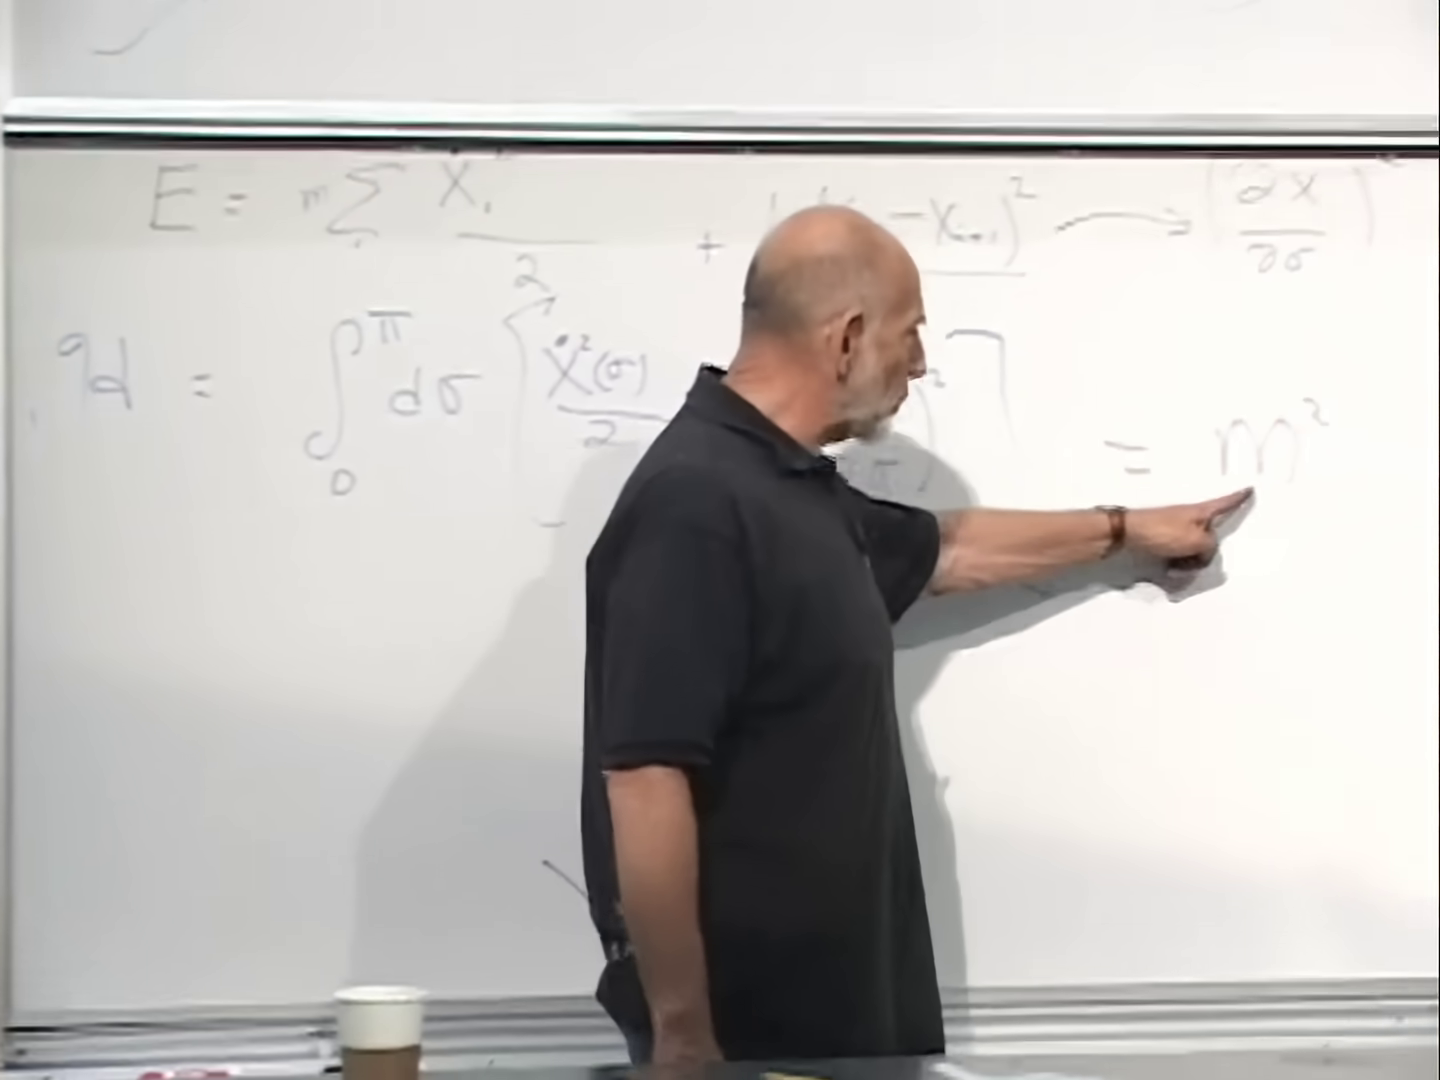
\includegraphics[width=0.76\textwidth]{lecture_01_figure_13.png}
  \caption{板书将内部弦能量等同于完整弦态的质量平方。}
  \lectureframe{01:10:30}
  \label{fig:l01-mass-squared-board}
\end{figure}

振动的弦是一组耦合振子。它的完整量子化被推迟了，但重要的谱结构事实已经可见。谐振子的能量以离散的台阶上升。由于这些内部能量对\(M^2\)有贡献，弦的激发自然会在质量平方中产生离散的台阶。这正是雷吉图在开头所预示的结构。

\begin{classroomqa}
\audiencequestion{\(M\)是整个弦的质量吗？如果将该质量加倍，相应的\(M^2\)贡献会变成四倍吗？
\lecturetimestamp{01:12:10}}
\lecturerresponse{是的。\(M\)是完整弦态的静止质量，包括振动、拉伸以及所有其他内部贡献。有效助推哈密顿量正比于\(M^2\)，因此质量加倍的态具有四倍的质量平方值。}
\end{classroomqa}

\begin{classroomqa}
\audiencequestion{这个描述如何能包含静止质量为零的光子？\lecturetimestamp{01:12:52}}
\lecturerresponse{无质量态对应于\(M=0\)。正的振子贡献如何能组合产生这样的态，是量子化理论的一个重要问题，而不是这里的经典模型所能解决的。在这一点上，\(M\)仅仅表示总静止质量，而量子力学尚未被引入。}
\end{classroomqa}

现在将一根不动的弦均匀拉伸到物理长度\(L\)。动能项消失，而在长度为\(\pi\)的参数区间上，

\begin{equation}
  \left|\partial_\sigma\bm X\right|\simeq\frac{L}{\pi}.
\end{equation}

因此，

\begin{align}
  H_{\mathrm{stretch}}
  &\propto
  \int_0^\pi d\sigma
    \left(\partial_\sigma\bm X\right)^2
  \notag\\
  &\simeq
  \pi\left(\frac{L}{\pi}\right)^2
  \propto L^2.
  \label{eq:l01-hooke-l2}
\end{align}

\begin{figure}[H]
  \centering
  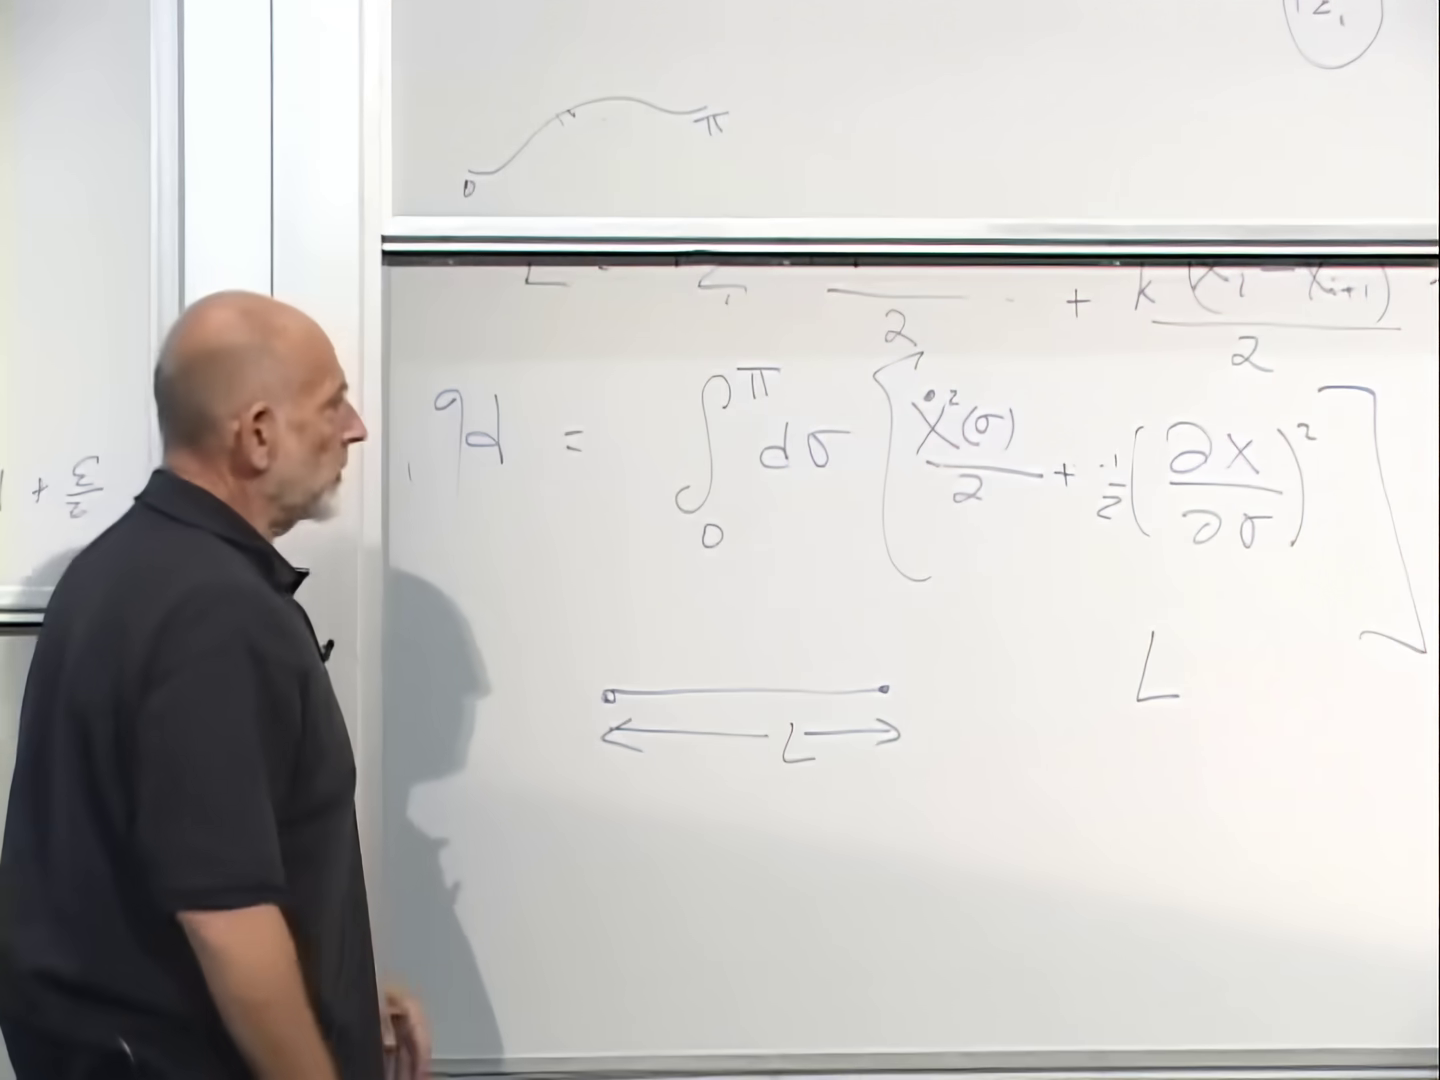
\includegraphics[width=0.76\textwidth]{lecture_01_figure_14.png}
  \caption{用于推断\(H_{\mathrm{stretch}}\propto L^2\)并进而推断\(M\propto L\)的均匀拉伸构型。}
  \lectureframe{01:15:30}
  \label{fig:l01-length-relation-board}
\end{figure}

这是有效横向力学中的胡克定律行为。但左边的量正比于\(M^2\)，而不是\(M\)。由此可得

\begin{equation}
  M^2\propto L^2,
  \qquad
  M\propto L.
  \label{eq:l01-mass-length}
\end{equation}

在静止系中能量为\(E_{\mathrm{rest}}=M\)，单位取\(c=1\)。将比例常数写为弦张力\(T\)，

\begin{equation}
  E_{\mathrm{rest}}=TL.
  \label{eq:l01-string-tension}
\end{equation}

结果与通量管图像一致。均匀的电场或磁场携带均匀的能量密度。如果其通量被限制在固定截面的管中，每增加一个单位长度就增加相同的能量。等价地，在新打开的每个间隙中填入新自由度的组分图像具有固定的单位长度能量。弦张力就是该单位长度能量。

这个结论是间接的。它并不声称任意被驱动到相对论速度的橡皮筋会自动获得\(E=TL\)。论证从大助推所导致的横向非相对论描述开始，将其内部能量等同于\(M^2\)，然后才将结果转换回静止系能量。

\section{同一物体在两个参考系中}

\(M\)与\(M^2\)之间的区别很容易被混淆，因此值得将两个展开式并排放置。取\(c=1\)，

\begin{align}
  E&=\sqrt{p^2+M^2}
  \simeq M+\frac{p^2}{2M},
  &&p\ll M,
  \label{eq:l01-rest-expansion-again}\\
  E&=\sqrt{P_z^2+M^2}
  \simeq P_z+\frac{M^2}{2P_z},
  &&P_z\gg M.
  \label{eq:l01-boost-expansion-again}
\end{align}

\begin{figure}[H]
  \centering
  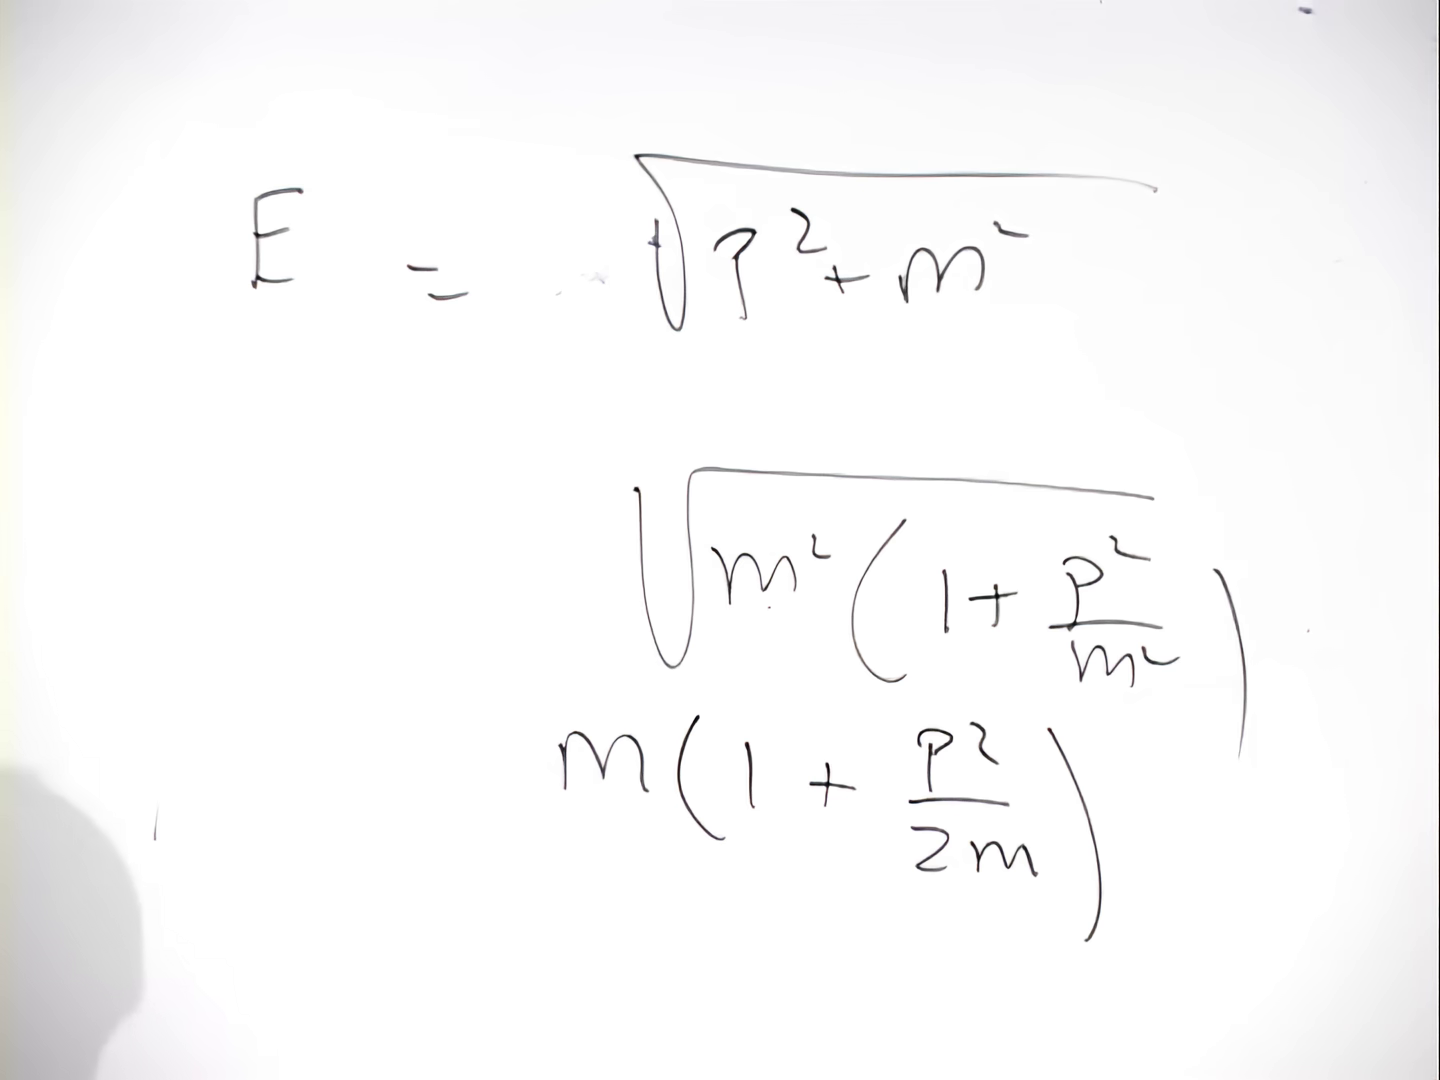
\includegraphics[width=0.74\textwidth]{lecture_01_figure_15.png}
  \caption{在分隔之后重复的小动量展开，其中内部静止能量被读作\(M\)。}
  \lectureframe{01:28:00}
  \label{fig:l01-rest-expansion-board-again}
\end{figure}

\begin{figure}[H]
  \centering
  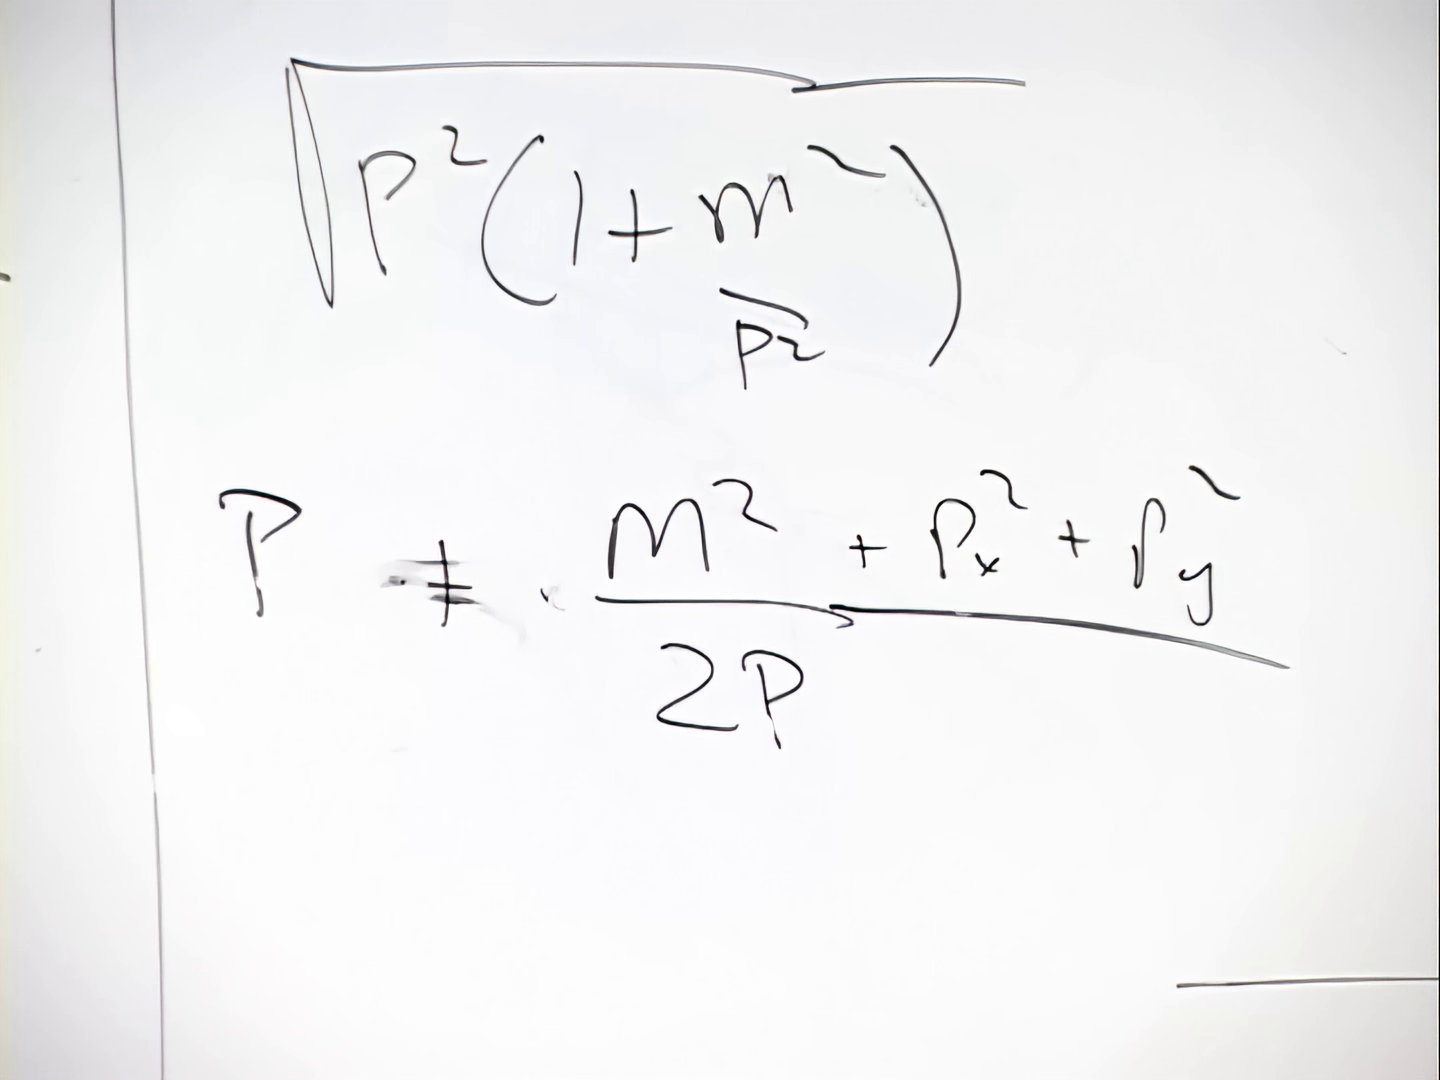
\includegraphics[width=0.74\textwidth]{lecture_01_figure_16.png}
  \caption{互补的大动量展开，其中剩余能量正比于\(M^2/(2P_z)\)。}
  \lectureframe{01:31:00}
  \label{fig:l01-boost-expansion-board-again}
\end{figure}

第一个展开将静止能量等同于质量，将普通惯性等同于\(M\)。在第二个展开中，守恒的\(P_z\)项被移除，横向惯性为\(P_z\)，内部能量由\(M^2/(2P_z)\)表示。无论在哪一个参考系中，质量都保持正比于弦长。变化的是质量的哪一个函数作为剩余哈密顿量出现。

\begin{classroomqa}
\audiencequestion{洛伦兹助推不应改变物理。为什么被助推的弦似乎服从不同的能量定律？
\lecturetimestamp{01:25:35}}
\lecturerresponse{它并不服从不同的物理。在两种描述中都有\(M\propto L\)和\(M^2\propto L^2\)。在静止系中，相关的能量是\(M\)；在大助推之后，守恒的\(P_z\)被分离出去，剩余的哈密顿量正比于\(M^2\)。助推改变的是有用的描述，而不是不变质量--长度关系。}
\end{classroomqa}

\section{一个超导的禁闭模型}

超导体将磁场从其体内排出。如果在材料变为超导态之前，磁通量被俘获在足够狭窄的通道中，那么磁通量就无法向侧面扩散，而是被限制在一根管中。一个有用的思想实验是：在正常态样品上钻一个窄孔，将一根长条形磁铁插入其中，冷却样品，然后抽出磁铁。这一构造是示意性的，而非实用的实验室操作方案。其目的是隔离出一条磁通线，使其场强和能量密度沿其长度方向近似均匀。

\begin{figure}[H]
  \centering
  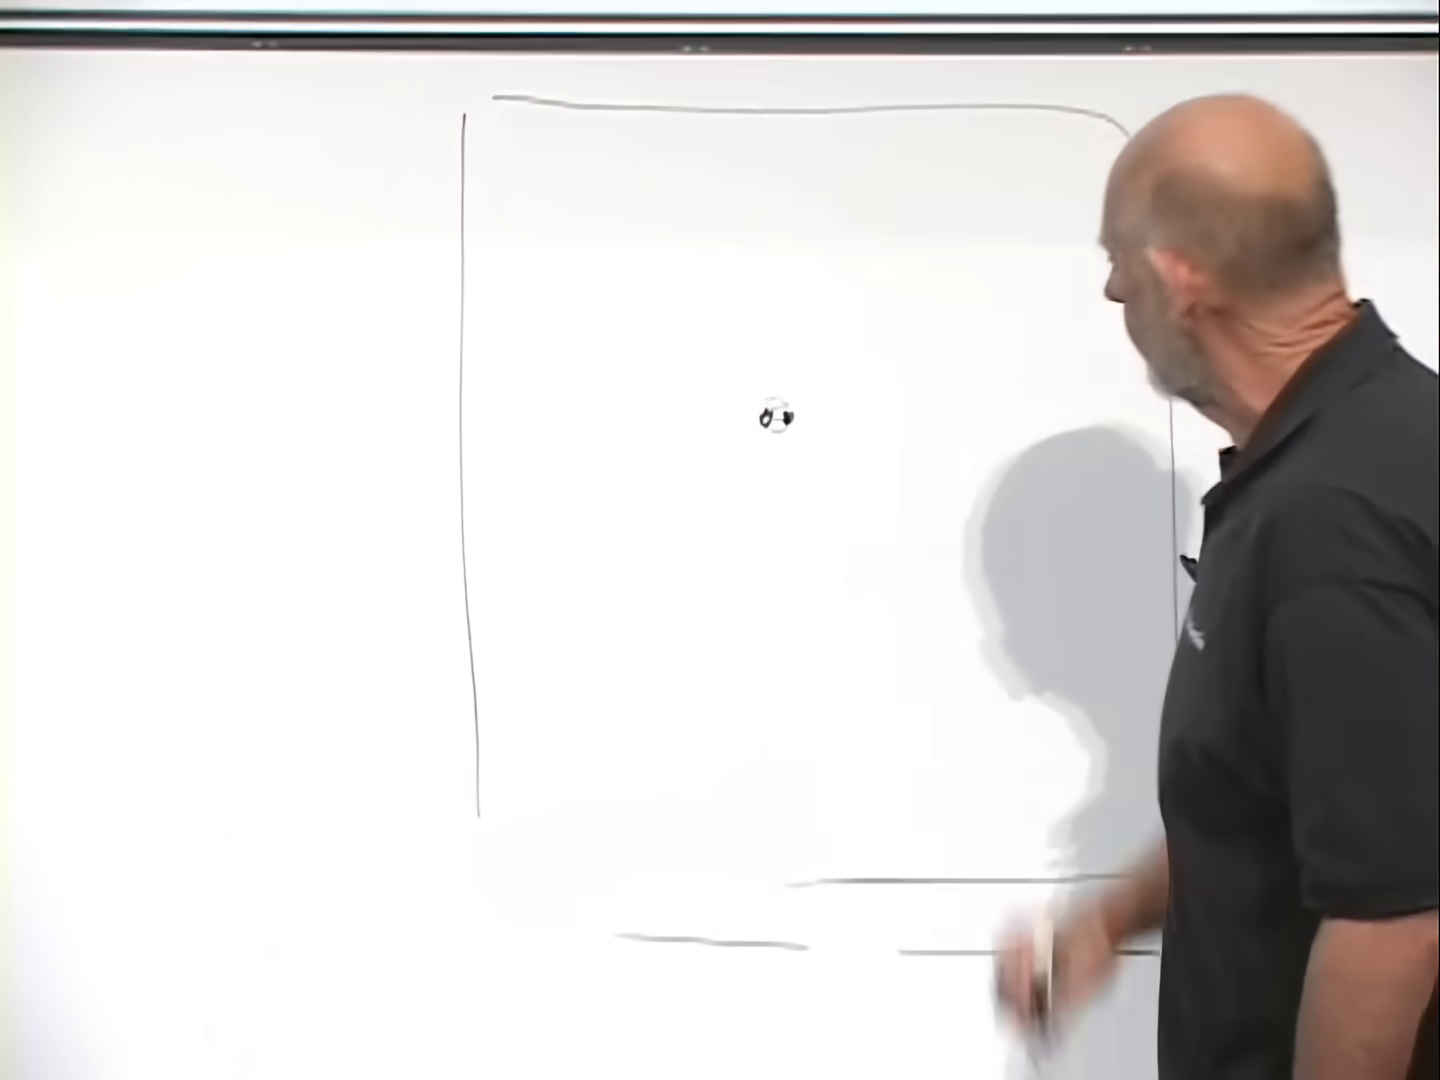
\includegraphics[width=0.76\textwidth]{lecture_01_figure_17.png}
  \caption{超导磁通线构造以及相应的单极子--反单极子禁闭图像。}
  \lectureframe{01:35:30}
  \label{fig:l01-superconductor-board}
\end{figure}

作为进一步的思想实验，假设可以将一个磁单极子和一个反单极子置于超导介质中并使其分离。它们之间的磁通量将被挤压成一根管。由于管每单位长度携带相同的能量，

\begin{equation}
  V(R)=T_{\mathrm{flux}}R.
  \label{eq:l01-linear-confinement}
\end{equation}

力 \(F=-dV/dR\) 的大小恒定。将这对粒子拉开变得越来越费力，因此这对粒子被禁闭。这正是人们为强子中的夸克所寻求的行为。

\begin{figure}[H]
  \centering
  \begin{tikzpicture}[>=Latex]
    \fill[blue!8,rounded corners=5pt] (-4,-1.35) rectangle (4,1.35);
    \node[blue!55!black] at (0,1.65) {superconducting medium};
    \fill[red!75!black] (-2.8,0) circle (0.17);
    \fill[blue!70!black] (2.8,0) circle (0.17);
    \node[below] at (-2.8,-0.22) {monopole};
    \node[below] at (2.8,-0.22) {antimonopole};
    \fill[orange!18,rounded corners=7pt] (-2.65,-0.42) rectangle (2.65,0.42);
    \draw[orange!85!black,thick,rounded corners=7pt]
      (-2.65,-0.42) rectangle (2.65,0.42);
    \foreach \y in {-0.22,0,0.22}
      \draw[->,orange!85!black] (-2.55,\y) -- (2.55,\y);
    \draw[<->] (-2.8,-1.00) -- (2.8,-1.00) node[midway,below] {$R$};
  \end{tikzpicture}
  \caption{磁通禁闭给出均匀的管和线性势
  \(V(R)=T_{\mathrm{flux}}R\)。}
  \label{fig:l01-superconductor-redraw}
\end{figure}

\begin{classroomqa}
\audiencequestion{在强子中，什么扮演了超导介质的角色？\lecturetimestamp{01:36:57}}
\lecturerresponse{所提出的类比将电和磁的角色互换。普通的超导凝聚体是带电的，并禁闭磁通量。在QCD的对偶超导体图像中，色磁物体的凝聚体禁闭夸克的色电荷。这类物体不会作为孤立粒子出现，因为它们被表示为凝聚在真空中。}
\end{classroomqa}

\editorialnote{对偶超导体描述是一种有影响力的禁闭机制，此处以讲座的历史性语言呈现。它应被理解为QCD真空的一种物理图像，而非从第一性原理出发对禁闭的完整推导。}

\begin{classroomqa}
\audiencequestion{能量与长度成正比，对于任何被高度相对论化的普通弦来说，这是一条普遍规则吗？\lecturetimestamp{01:38:10}}
\lecturerresponse{不是。人们首先需要一种关于该材料的自洽的相对论性理论，而其行为将取决于具体细节。线性能量是如下构型的特殊性质：其密度在被延伸时保持固定，或者磁通量被阻止横向扩散。将其拉开会产生更多的组分或更多均匀充满场的长度，而不仅仅是增大一组固定分子之间的间距。}
\end{classroomqa}

\section{横向自由度与粒子的尺度}

光锥构造直接以弦的横向坐标来书写弦。并不存在与每个横向振子相对应的、可独立指定的纵向振子。这种直接空间维度减少一个的现象是该形式体系的显著特征之一；不过，完整的理论仍必须满足洛伦兹不变性。

\begin{classroomqa}
\audiencequestion{沿 \(z\) 方向的剩余运动会发生什么？
\lecturetimestamp{01:40:10}}
\lecturerresponse{在光锥描述中，纵向运动不是作为独立自由度引入的。物理振荡由横向描述，而约束条件决定了纵向信息。这种经济性与如下想法在精神上相关：引力系统或许允许一种直接维度少一个的描述，尽管此处并未推导这一联系。}
\end{classroomqa}

\begin{classroomqa}
\audiencequestion{雷吉图上实际已知多少个点？
\lecturetimestamp{01:41:15}}
\lecturerresponse{确切的最大值取决于家族；粗略的数字大约是七个。这一序列在实验上并非无穷无尽。相关的事实是，已知的点并未显示出普通宏观材料中那种可见的失效或断裂端点。}
\end{classroomqa}

强子现象学提供了历史动机，但数学弦理论并不需要复现强子的每一个细节。一旦形式体系建立起来，人们就会问它实际上描述了什么。它的无质量自旋二态和其他性质更自然地指向引力。

强子与电子之间的表面差异可以用刚性转动的能量来量化，

\begin{equation}
  E_{\mathrm{rot}}=\frac{J^2}{2I},
  \qquad
  I\sim MR^2.
  \label{eq:l01-rotational-energy}
\end{equation}

角动量是量子化的。将 \(J^2\) 示意性地写作 \(\hbar^2 n^2\)，第一个转动台阶的量级为

\begin{equation}
  \Delta E_{0\to1}\sim\frac{\hbar^2}{2I}.
  \label{eq:l01-first-rotational-step}
\end{equation}

\begin{figure}[H]
  \centering
  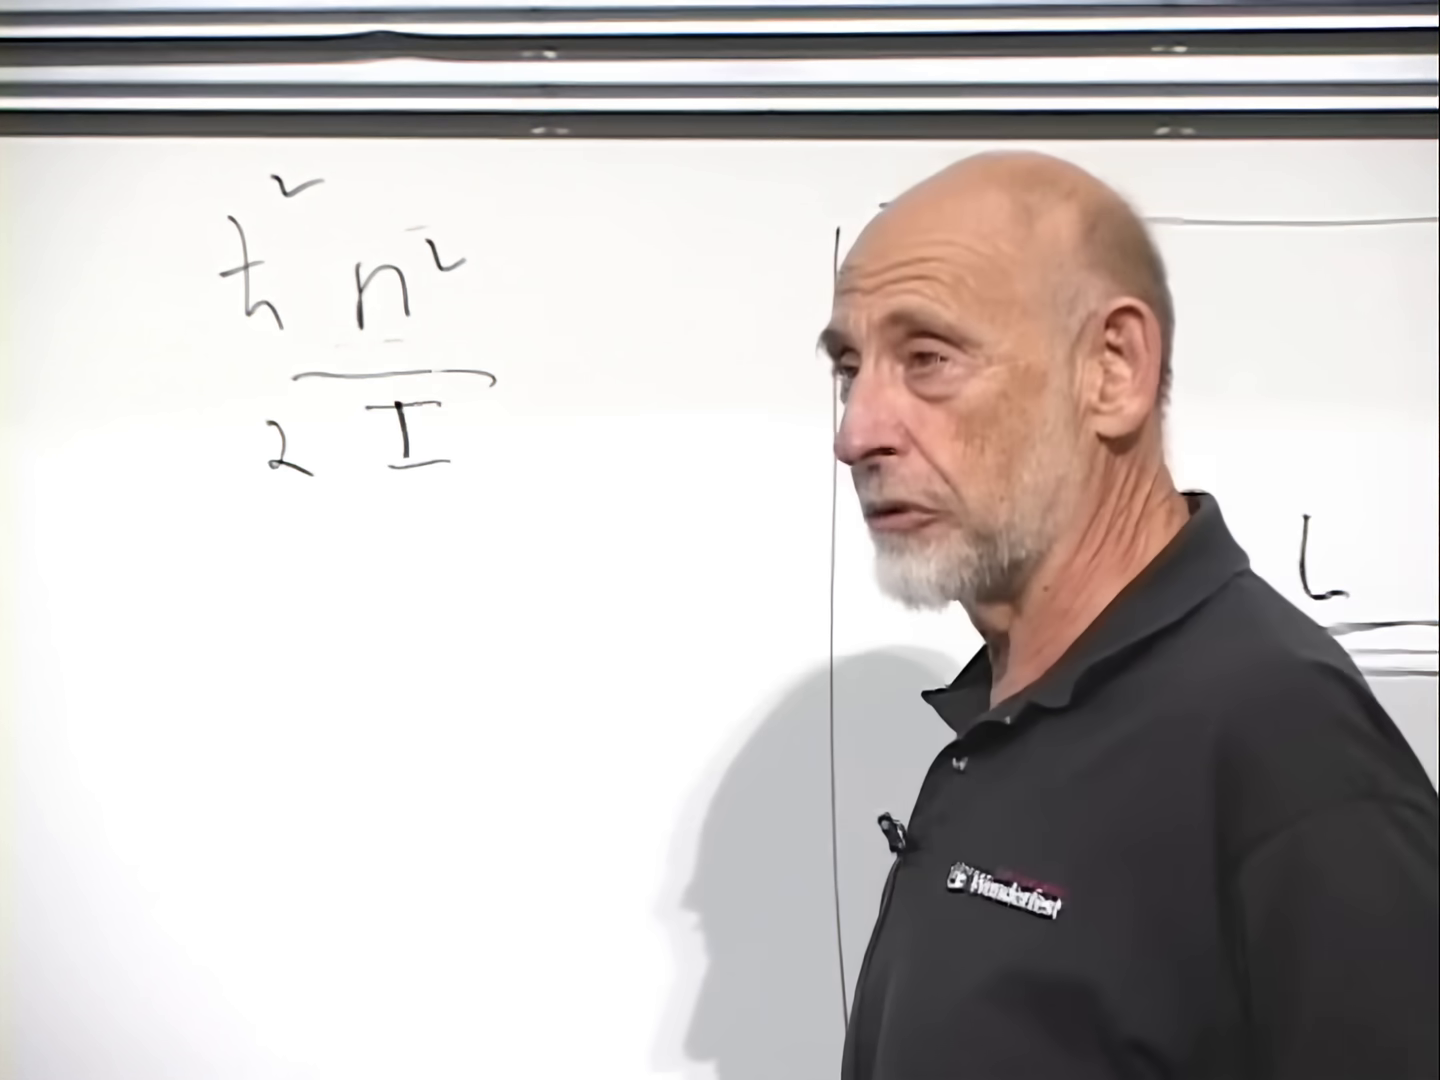
\includegraphics[width=0.76\textwidth]{lecture_01_figure_18.png}
  \caption{第一转动激发的转动惯量估计，\(\Delta E\sim\hbar^2/(2I)\)。}
  \lectureframe{01:44:00}
  \label{fig:l01-rotational-board}
\end{figure}

对于固定质量，半径越小意味着转动惯量小得多，而激发能量大得多。强子在自身内部动力学的尺度上很大，因此一次转动激发大约需要一GeV的能量，在粒子碰撞中是可以达到的。如果电子具有任何空间子结构，实验限制使其尺度远小于此，而转动激发将远超出可获得的能量范围。篮球则处于相反的极端：其转动惯量如此之大，以至于一个角动量量子所需的能量小得无法察觉。原子的转动或轨道能级跃迁介于这些极端之间，通常在电子伏特的量级。

\begin{classroomqa}
\audiencequestion{一个看似基本的电子是否仍可能具有空间结构和转动激发？\lecturetimestamp{01:42:04}}
\lecturerresponse{它只能将它们隐藏在非常高的能量处。一个单位角动量的代价按\(1/I\)标度，而\(I\sim MR^2\)。因此，极小的半径会将第一激发推到质量平方图上很远的地方。未观察到电子激发意味着，要么电子是点状的，要么任何复合尺度都远小于当前实验所能分辨的尺度。}
\end{classroomqa}

现在可以从动力学角度解读开篇的Regge图。强子之所以展现出可及的转动和振动状态，是因为它们是延展的。其质量平方谱中的等间距步长，正是将振子哈密顿量等同于\(M^2\)时所预期的特征。其能量随长度近似线性变化，是恒定张力通量管的特征。光谱学、散射对偶性、世界面几何和光锥力学，是对同一个组织性思想的四种描述：一个延展的相对论性客体，其自然的内部变量是质量平方。
